\chapter{Aggregation Models}
\label{chap:potts_aggregation}

\section{Introduction and Motivation}
As we have seen in the previous chapters, the folding properties of a single protein are not only affected by the surrounding solution, but also the conformational state space available through confinement and excluded volume interactions. Up until this point we have considered the protein folding process as an independent event, including only an entropic solute interaction. In reality, there exist multiple biological events that feature enthalpic protein-protein interactions. Focusing on a subset, we apply our techniques to the study of aggregated species to model proteins that form composite structures which are larger and more complex than the sum of the individual elements.

Our study of aggregated species is primarily motivated by the devastating neurodegenerative disorder known as Alzheimer's disease. Alzheimer's is a progressive disorder that causes a deterioration of memory and cognitive function. The disease is the leading cause of dementia,\cite{querfurth_alzheimers_2010} effecting over thirty-five million people worldwide. The principal risk factor for contracting the disease is age, with the incidence doubling every five years after age 65. At 80 years old, one in six people have the disease.

Plaques of amyloid-$\beta$ (A$\beta$) fibrils are recognized as an important pathological feature in Alzheimer's disease. At normal physiological parameters, A$\beta$  is known to spontaneously self-aggregate into oligomers of two to six peptides. These in turn coalesce into larger forms. A$\beta$ can then grow into fibrils that form insoluble $\beta$-pleated sheets of amyloid plaques. However, it is the soluble oligomers and smaller amyloids that have been shown to be the most neurotoxic. This is evidenced by correlating the levels of the oligomerization with toxicity to synapses in brain-slice preparations.\cite{walsh_certain_2005} This is interesting, since the total amount of A$\beta$ plays less of a role than the intermediate growth phase.\cite{lue_soluble_1999} Structural information for the A$\beta$ peptide and its oligomers and fibril structure has been slow,\cite{kajava_beta-structures_2006} but recent results are beginning to emerge that detail these key features of the aggregation process.\cite{streltsov_crystal_2011} What is needed, is a general model that can incorporate these findings for A$\beta$ and other aggregation problems.  Aggregation studies of these proteins, and indeed all proteins in general, are essential to our understanding of the disease.

It is the aim of this chapter to develop and investigate several aggregation models with the tools introduced in this thesis. We begin with Section \ref{sec:first_order_aggregation}, where we develop a simplified first-order model. In it, we make several simplifying assumptions on the conformations and energies of the aggregated species. While the model is useful to develop intuition, we find that it is too restrictive and unable to provide a complete description about the aggregation process. To that end we generalize the first-order model in Section \ref{sec:potts_over_arbit_graphs} by reformulating the aggregation problem as the Potts model in an external field over an arbitrary graph. The main result of this chapter is the development and application of this solution as an operator expansion. With this method we are able to present new results on the Potts model problem. In Sections \ref{sec:one_d_ladder} and \ref{sec:two_d_ladder} we derive results for a one-dimensional `ladder' with thickness one and two respectively. Finally we present results in Section \ref{sec:edge_contraction_methods} for a wider class of problems with a subgraph recursion relation, albeit in the absence of external fields.

\section{First-order Aggregation}
\label{sec:first_order_aggregation}

Just as we coarse-grained the amino acid residues in Chapter \ref{chap:WL_crowding} to study the folding properties of a single protein, as we study the aggregation process we will make a suitable approximation for the larger length scale of aggregated species. In this section we will approximate an entire protein as one unit on a graph or lattice. Aggregation then, is a study of nearest neighbor contacts over this graph. 

Consider a simple interaction model over a square lattice with side length $L$ and $N=L^2$ sites with the Ising Hamiltonian
\begin{equation}
\HAM = -J \sum_{\avg{i j}} \sigma_i \sigma_j
\end{equation}
The lattice spacing is such that only a single particle can be occupied at any given site, hence $\sigma_i \in \{0,1\}$ corresponds to a lattice site being occupied or not. The interaction strength $J$, is related to the propensity for two proteins to be found next to each other. The summation extends over all nearest neighbors with a global restraint on the number of particles in the system $(m \leq N)$
\begin{equation}
\sum_i \sigma_i = m 
\end{equation}
Ultimately we want to set $N \rightarrow \infty$ corresponding to the thermodynamic limit. Thus we scale the interaction strength with the number if lattice sites as
\begin{equation}
J \propto \ln N
\label{eq:first_order_aggregation_scaling}
\end{equation}
%
The object of our study is a cluster or an oligomer, a collection of $m$ proteins that are connected through a path of nearest neighbors. For a given $m$ we partition the cluster configurations into combinations of clusters of different sizes and shapes. For example if $m=3$ we consider the partitions $[1,1,1], [1,2], [3]$ which correspond to 3 monomers, a monomer and a dimer, and a trimer, respectively. To the leading order in powers of $N$, the number of ways these configurations can be placed on the lattice are $N^3, N^2$ and $N$, respectively. We assume an individual $k$-mer is compact, it always its lowest energy state. On a 2D lattice this corresponds to an energy as a function of the cluster size $k$ 
\begin{equation}
 \HAM(k) = J \piecewisebrace{
 \begin{array}{lll}
   k + \lfloor k/2 -2 \rfloor & : & k > 1\\
   0                          & : & \text{otherwise}
 \end{array}
 }
\label{eq:piecewise_aggregation_eq_ham}
\end{equation}
%
where $\lfloor x \rfloor$ is the floor function. The partition function can then be written as
\begin{equation}
\Z = \sum_{p \in \text{partitions(m)}} N^ { \abs{p} }
\exp \paren{  - \beta { \sum _{k \in p} \HAM(k) } }
\end{equation}
This leads to several interesting properties. When $m$ is even it appears that there is a single first-order phase transition at $\beta_{1} = \frac{2m-2}{3m-4}$. When $m$ is odd and $m>3$ there are phase transitions at $\beta_{1}$ and $\beta_{2}=1$. These phase-transitions happen as the spontaneous collapse of the roots of a $m^{\text{\tiny th}}$ order polynomial equation. The type of phase-transition is logarithmic in $N$. 

\subsection{First-order pentamer model}
We illustrate the method with a worked example of the first-order theory with $m=5$. The set of partitions of $5$ particles (monomers to pentamers) is given by
\begin{equation}
\text{partitions}(5) = \{ [1,1,1,1,1],[1,1,1,2],[1,2,2],[1,1,3],[2,3],[1,4],[5] \}
\end{equation}
The energy of a single polymer in its configuration of maximally compact shape is given by Equation \ref{eq:piecewise_aggregation_eq_ham}: the monomers have energy proportional to 0, dimers 1, trimers 2, tetramers 4, 5-mers 5. Scaling the energy as in Equation 
\ref{eq:first_order_aggregation_scaling}, this gives the partition function as
\begin{equation}
\Z={N}^{5}+{N}^{4}{{\rm e}^{{ \beta}\,\ln  N }}+2\,{N}^{
3}{{\rm e}^{2\,{ \beta}\,\ln  N }}+{N}^{2}{{\rm e}^{3
\,{ \beta}\,\ln  N }}+{N}^{2}{{\rm e}^{4\,{ \beta}
\,\ln  N }}+N\,{{\rm e}^{5\,{ \beta}\,\ln  N
  }}
\label{eq:part_func_first_order_n_5}
\end{equation}
Using units where $k_B = 1$, the specific heat is $C_V = \beta^2 \pfrac{^2}{\beta ^2} \ln \Z$, we seek the discontinuities of $C_V$ as $N \rightarrow \infty$. Dropping the factor of $\beta^2$ this amounts to finding the discontinuities $C_V(\beta_C) = \infty$
\begin{equation}
\beta_C = \lim _{N \rightarrow \infty} \frac{1}{\ln N} \ln (\text{Roots}(f_5(x)) )
\end{equation}
with the polynomial $f_5(x)$ defined as
\begin{equation}
f_5(x) = n^5 + n^4 x + 2 n^3 x^2 + n^2 x^3  + n^2 x^4  + n x^5
\label{eqn:Worked_5_example_polynomial}
\end{equation}
%
\begin{figure}[ht]
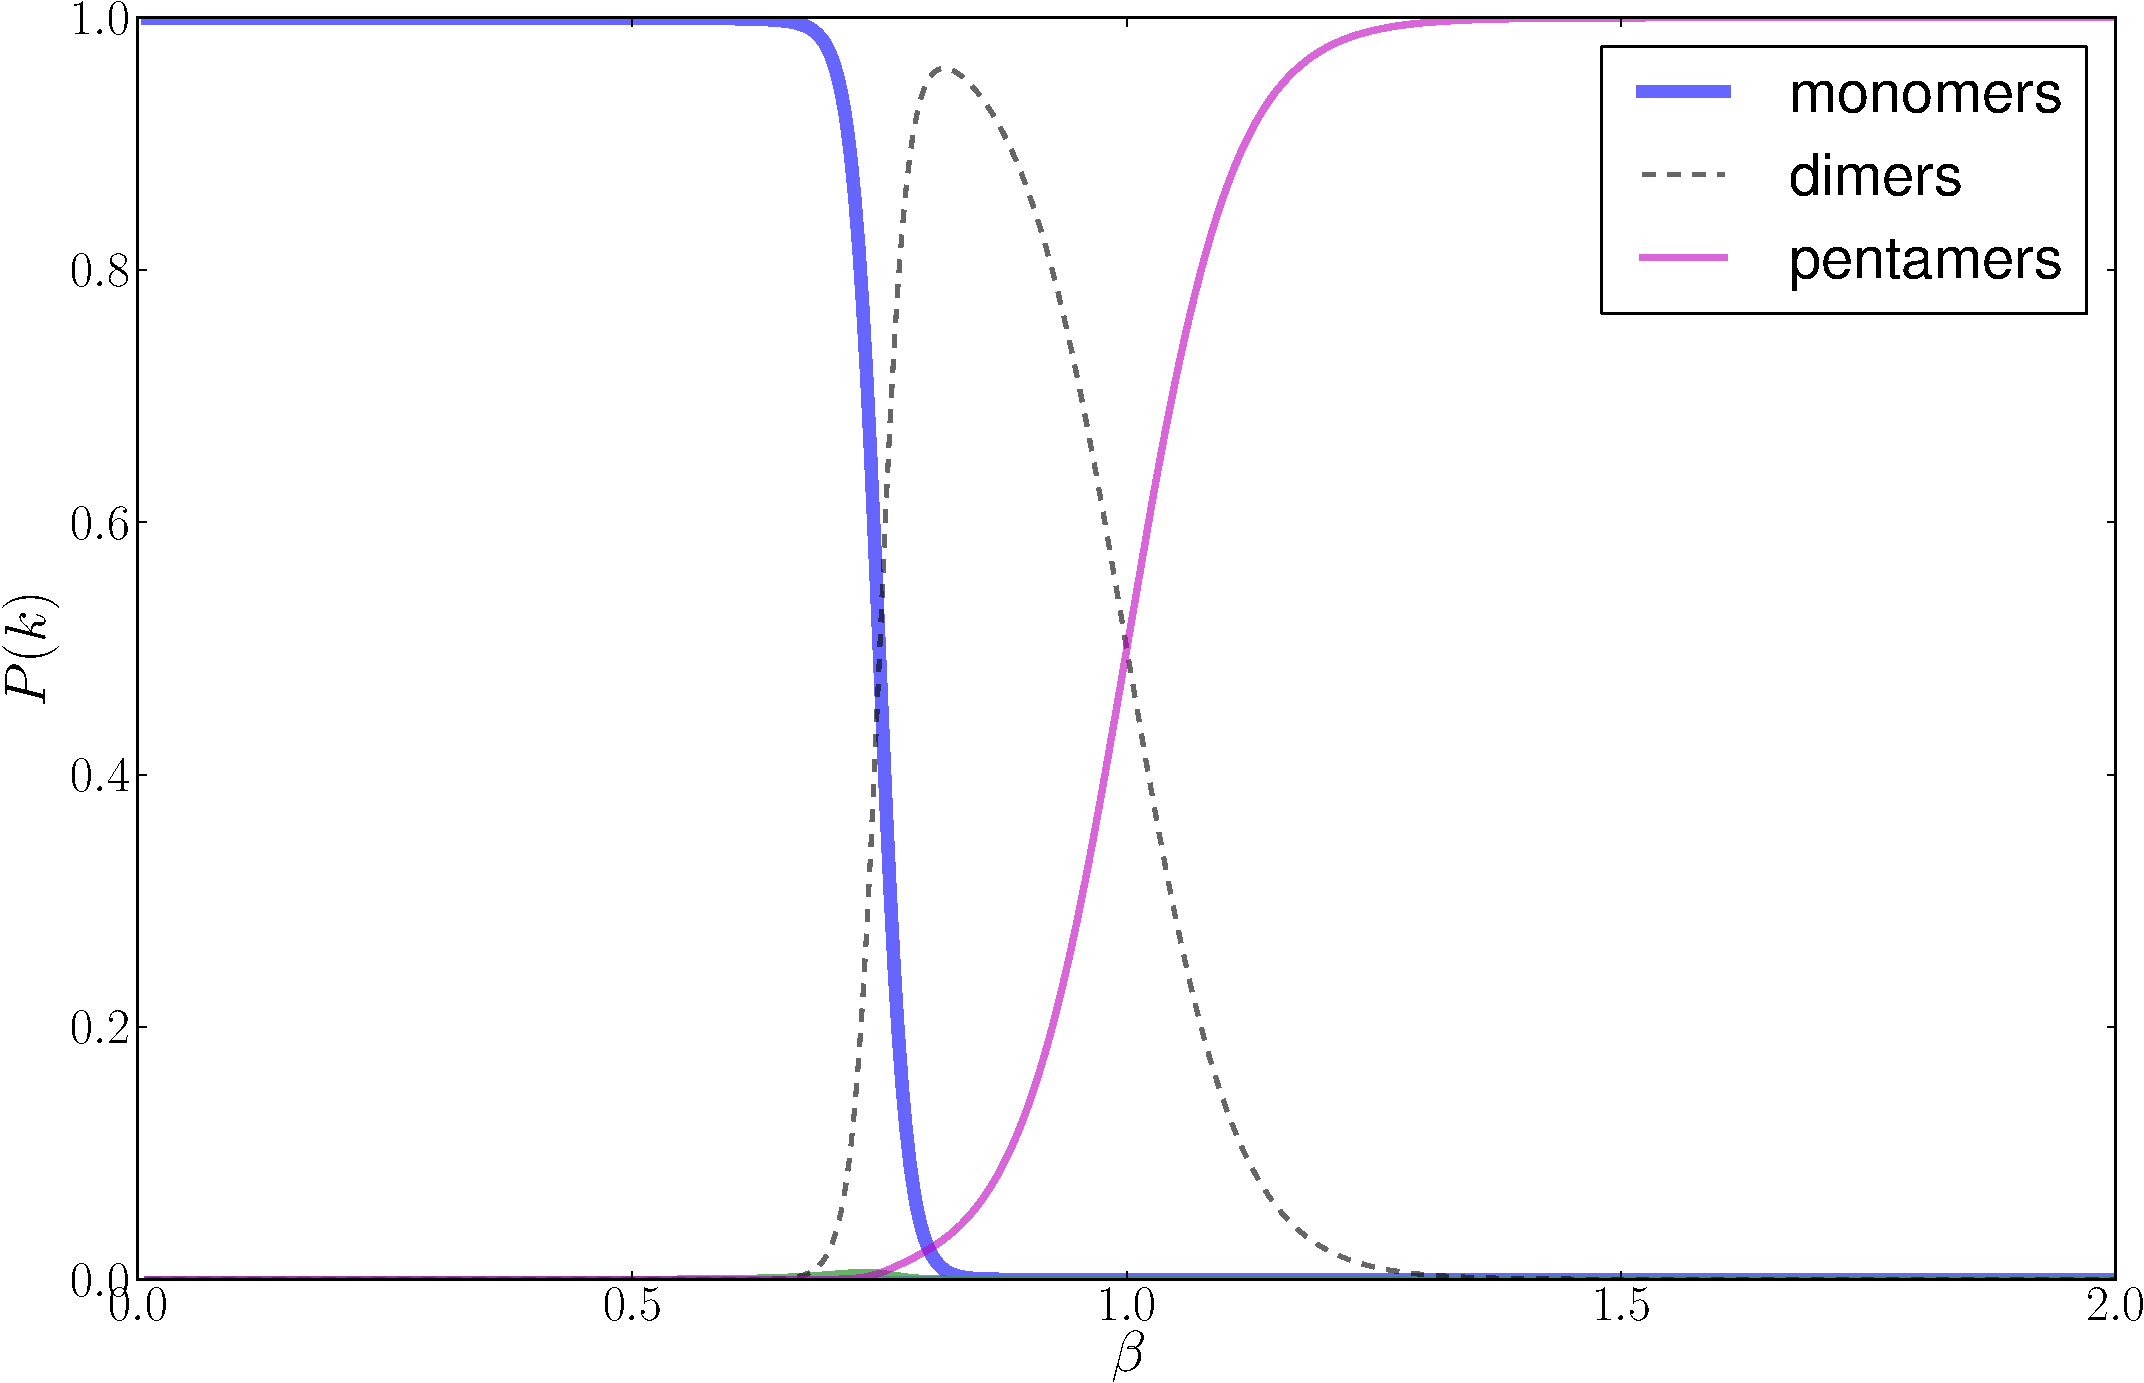
\includegraphics[width=.47 \textwidth]{pictures/aggregation_model/pictures/N=5_PZ.pdf}
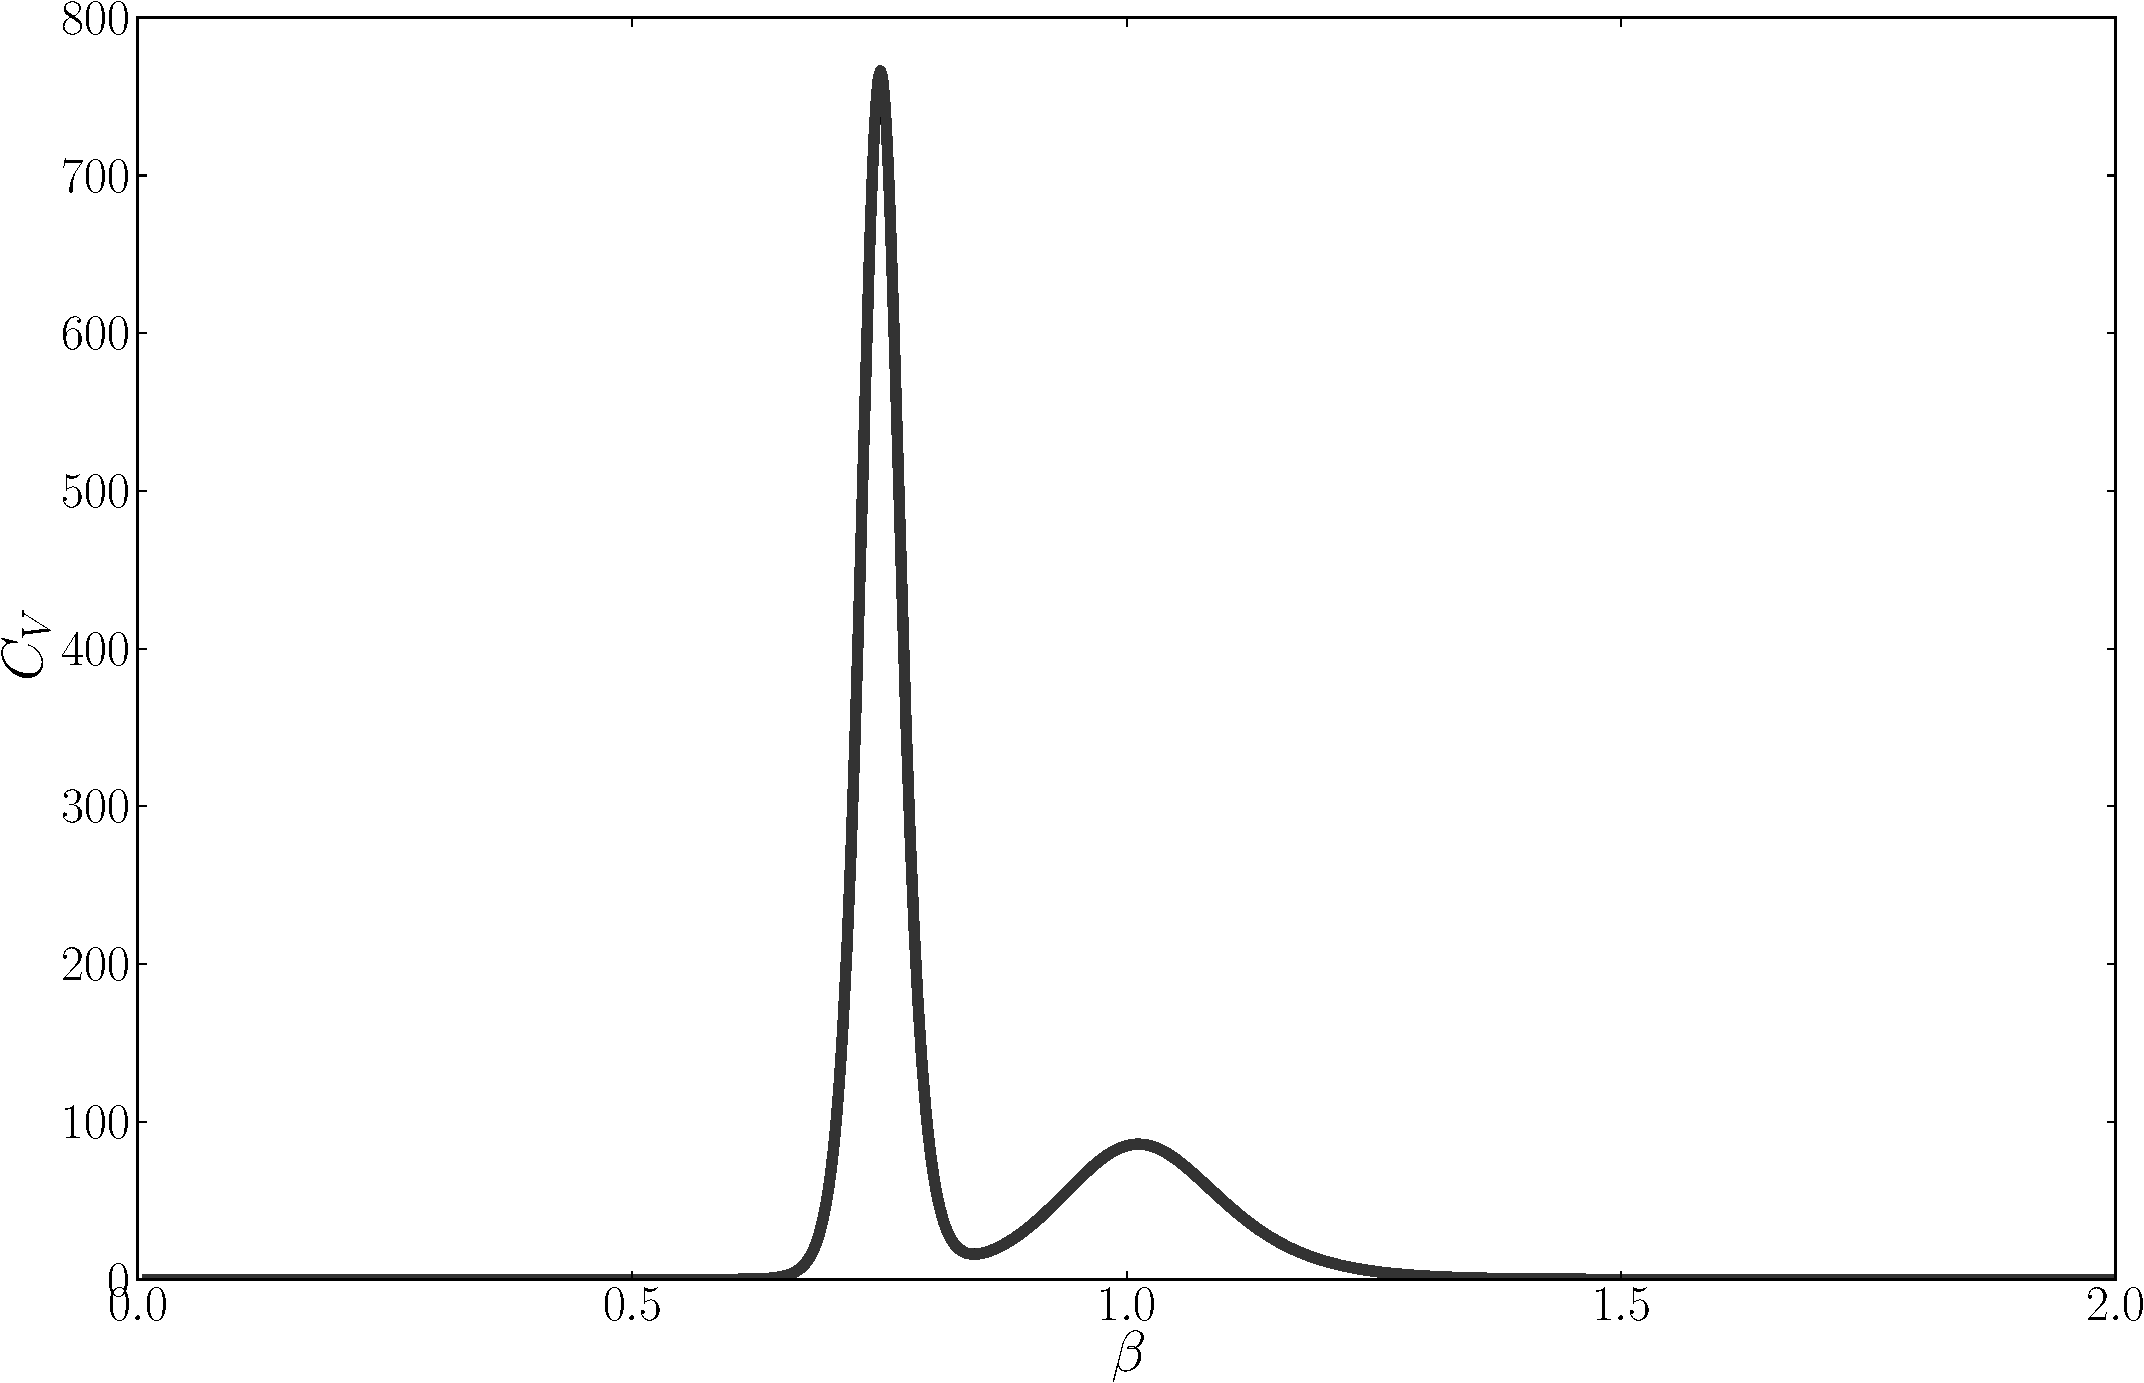
\includegraphics[width=.47 \textwidth]{pictures/aggregation_model/pictures/N=5_CV.pdf}
\caption{For the first-order aggregation model, the first graph shows the probability of each $k$-mer as a function of $\beta$ for the different conformations for the specific case of $m=5$. The second graph shows the specific heat as a function of $\beta$ for large $N$ ($N=10^{16}$). The large peak represents the first aggregation of monomers to dimers while the smaller peak signifies the collapse of the system to the lowest energy state of the pentamer. The trimers and tetramers have a low probability for all temperatures and are only visible near the transition temperature.}
\label{fig:Worked_5_example_picture}
\end{figure}
%
The coefficients to this polynomial come from the terms in the energy function. For this particular problem the solutions to equation \ref{eqn:Worked_5_example_polynomial} are
\begin{equation}
\beta_C = \braces{ 1, \frac{3}{4} }
\end{equation}
With a four-fold degeneracy on the $3/4$ root (see Figure \ref{fig:Worked_5_example_picture}). 

In the original work by Yang and Lee,\cite{lee_statistical_1952} they considered the grand partition function in terms of the fugacity. By extending the fugacity to the complex plane they used it to show that an Ising-like model will have complex roots on a unit circle. The expansion above is a continuation of this idea, except the parameter extended to the complex plane is $\beta$ and the zeros are known as Fisher zeros.\cite{fisher_1965_nature} In this case (as in many others), the zeros do not lie on a unit circle and produce intricate structures on the complex plane.

In Figure \ref{fig:zeros_part_func_first_order} we plot the phase angle of $\Z$ when temperature is continued onto the complex plane. The zeros of this function signify phase changes of the system. These zeros are visible on the complex plots by noting that around the poles the phase will change by a multiple of $2 \pi$. 

\begin{figure}[ht]
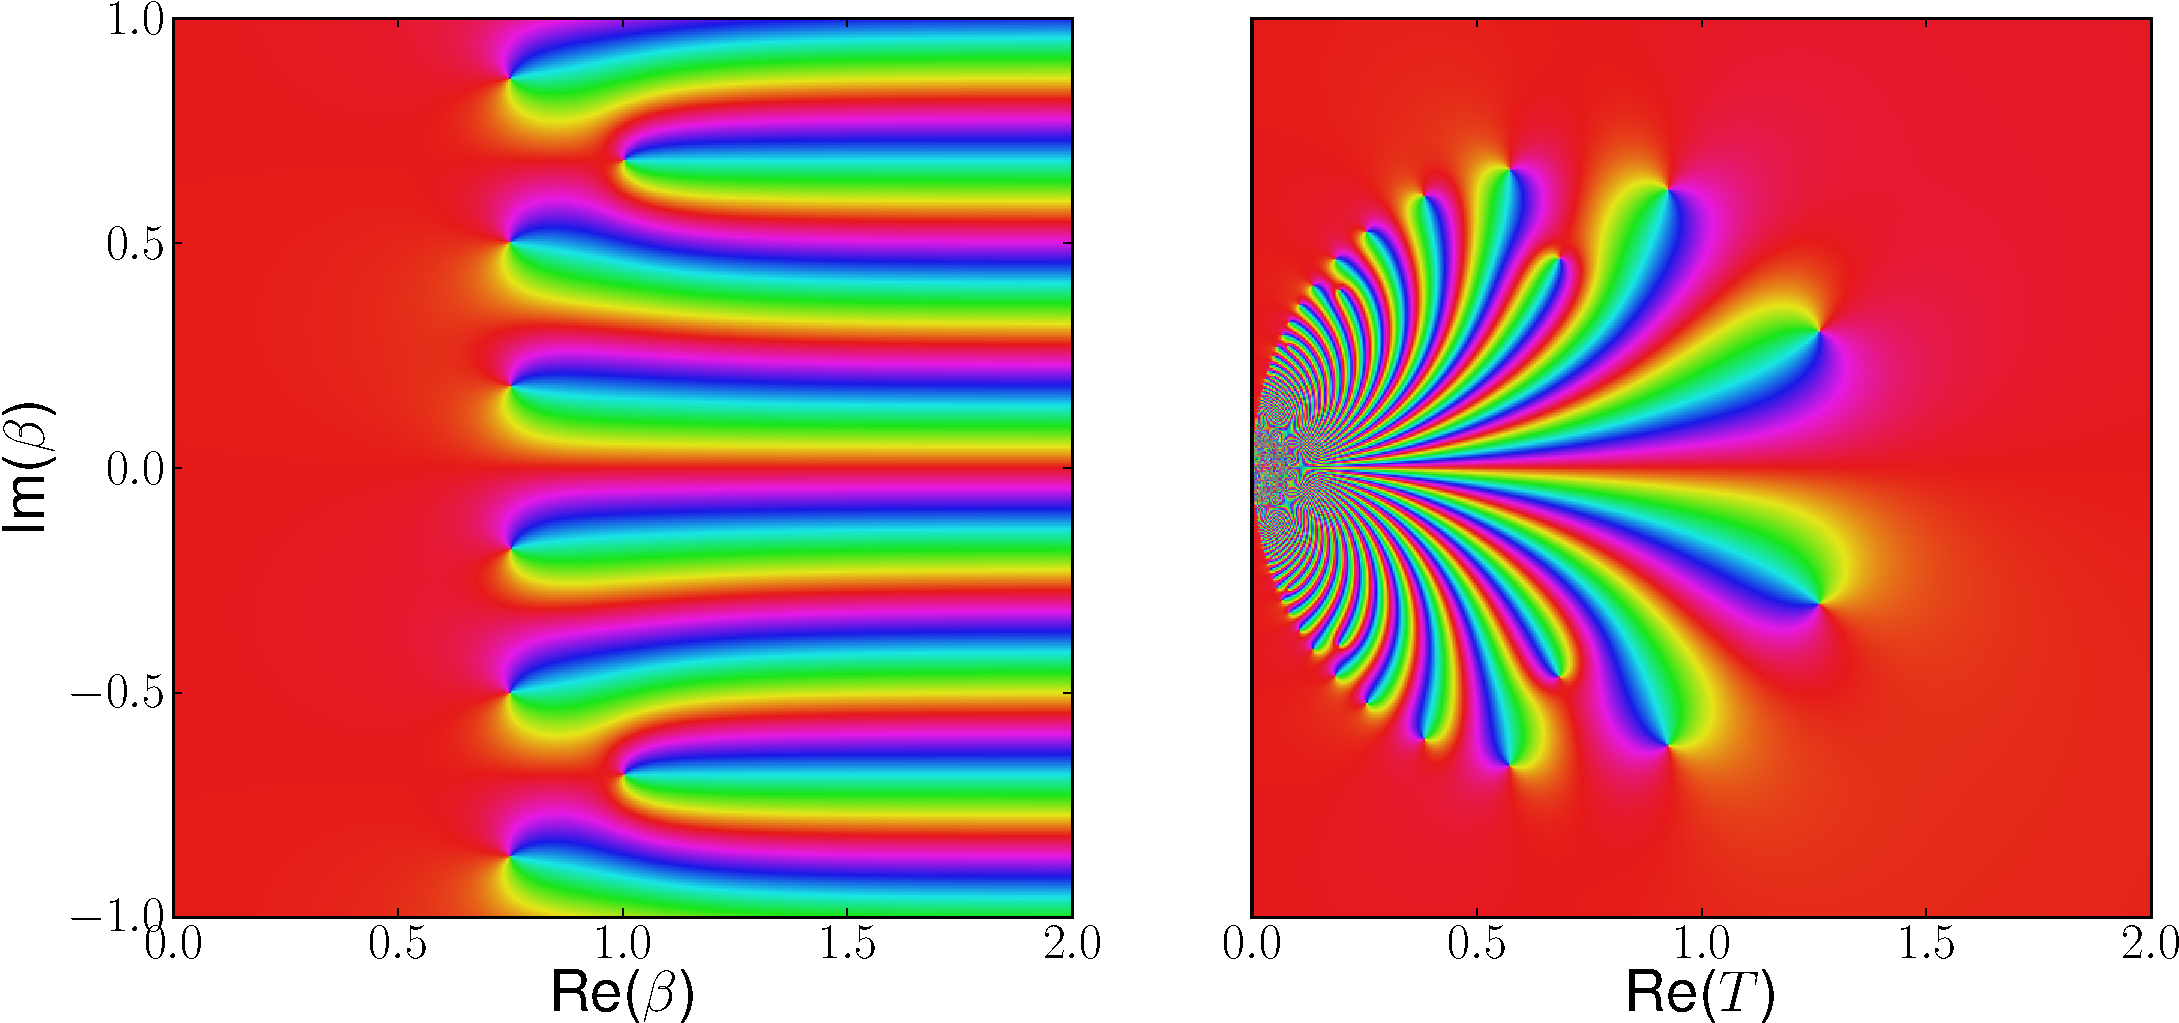
\includegraphics[width=\textwidth]{pictures/aggregation_model/pictures/f5_part_func_zeros.pdf}
\caption{Partition function of Equation \ref{eq:part_func_first_order_n_5} with $\beta$ analytically continued onto the complex plane. The colors of the graph mark the phase angle of the function, thus simple poles are marked by a complete change of color (due to Cauchy's theorem). The zeros at $\beta=1$ and $3/4$ can clearly be seen, but they have not yet collapsed onto the real plane due to finite $N$ (here $N=10^4$). Increasing $N$ alters the density of the zeros until they touch the real axis as $N$ goes to infinity.
}
\label{fig:zeros_part_func_first_order}
\end{figure}

We list the values of the function $f_n$ for several small $n$
{
\begin{align}
\label{eq:first_order_agg_series_list}
f_1(n) &= n 
\\ \notag
f_2(n) &= n^2+nx
\\ \notag
f_3(n) &= n^3+n^2x+nx^2
\\ \notag
f_4(n) &= n^4+xn^3+2x^2n^2+x^4n
\\ \notag
f_5(n) &= n^5+xn^4+2x^2n^3+x^3n^2+x^4n^2+x^5n
\\ \notag
f_6(n) &= n^6+xn^5+2x^2n^4+2x^3n^3+x^4n^3+x^4n^2+2x^5n^2+x^7n
\end{align}
}

\subsection{Drawbacks of the First-Order Model}

The model is interesting, but lacks the fidelity needed to model real aggregated proteins due to the approximations made. For one, the treatment of a protein as a single unit with uniform bond-strengths prevents the expression of any non-isotropic growth patterns. This is a severe limitation, as many fibril growths and aggregated species have a preferred growth direction after a minimal nucleation size. Along those lines, the assumption that the protein will aggregate only in the most compact and hence lowest energy conformation (via Equation \ref{eq:piecewise_aggregation_eq_ham}), may be valid for protein folding but is certainly invalid for many types of aggregated species. 

The scaling relation, Equation \ref{eq:first_order_aggregation_scaling}, was introduced in an ad-hoc manner to help retain a finite convergence of the critical temperatures. The motivating idea behind the approximations was to reduce the problem to the expression of a single polynomial whose properties could be studied analytically. Equation \ref{eq:first_order_agg_series_list} lists several values of the polynomial series $f_m$, but we did not find any interesting properties of the system. It is unknown if there is a deeper relation between this general aggregation model and this series.

Despite the shortcomings of this simple aggregation model, it provides an instructive tool to develop a more general method. To account for these approximations, we introduce more degrees of freedom into the system. We let the conformations take arbitrary shapes and potentials through a Potts model and define the boundary conditions by the graph the system is embedded in. We attempt to develop a solution to the Potts model over an arbitrary graph and discuss the possibilities this opens for modeling in the next section.


\section{Potts-Model over Arbitrary Graphs}
\label{sec:potts_over_arbit_graphs}

Computing the partition function $\Z$ of a model with short-range interactions is a standard problem in statistical mechanics. Indeed, the Ising/Potts model has attracted attention from fields as diverse as condensed matter to biophysics to economics.\cite{wu_potts_1982} The prototypical example is the Potts model, defined over a graph $G$ with $N$ vertices, edge set $\mathcal{E}$, and vertex set $\vec \sigma$.
%
\begin{equation}
\vec \sigma = \brackets{ \sigma_1, \sigma_2, \ldots, \sigma_N }
\end{equation}
%
Each vertex $\sigma_i \in \vec \sigma$ has a `spin' property.%
\footnote{
We use the term spin to keep with the original terminology of the Ising model. In our case the spin is not related to the electronic states of an atom, but rather a marker of the internal conformation states of the protein.}
%
In contrast to the Ising model, each spin can point in $q$ different directions
%
\begin{equation*}
\sigma_i \in \braces{ 1,2,3, \ldots, q } 
\end{equation*}
%
The Hamiltonian for the Potts model on a simple graph can be defined as
\begin{equation}
\HAM = - J \sum_{ \avg{ij} }  \delta(\sigma_i, \sigma_j)
       - h \sum_{ \avg{i} }  \delta(\sigma_i, \alpha) 
\label{eq:potts_model_ham}
\end{equation}
%
where the first summation goes over all edges, while the second summation goes over each vertex. Here $\delta$ is the Dirac delta function, $J$ is the strength of the bond interaction and $h$ is the strength of the external field (which acts only on spins pointing in direction $\alpha$). The system is fully specified by the arrangement of the spin at each vertex. Let $\sigma' \in \vec \sigma$ denote a particular set of spin conformations from the set of all arrangements. The partition function for the system is a sum over all such possible spin arrangements
\begin{equation}
\Z = \sum_{\sigma ' \in \vec \sigma} e^ { -\beta \mathcal{H}(\sigma ')  }
\end{equation}
%
We can expand the expression by noting that
\begin{align}
\label{eq:expanded_partition_function}
\Z &= 
      \sum_{\sigma ' \in \vec \sigma} 
      e^{ \beta J \sum_{\avg{ij}}  \delta(\sigma_i ' , \sigma '_j) }  
      e^{ \beta h \sum_{\avg{i}}   \delta(\sigma_i ' , \alpha) }  \notag\\
	&= \sum_{\sigma ' \in \vec \sigma}  
	\prod_{\avg{ij}} \brackets{ 1 + v \delta(\sigma_i ' , \sigma_j ' ) }
	\prod_{\avg{i}}  \brackets{ 1 + u \delta(\sigma_i ' , \alpha) }
	\notag
\end{align}
%
With the understanding that $v = e^{\beta J} - 1$, and $u = e^{\beta h} -1$. This gives a polynomial in $u$ and $v$ that reduces down to several other well known polynomials such as the Tutte and chromatic polynomial.\cite{godlin_graph_2008}

By definition, the partition function is the weighted sum over all possible states. Quite often physical problems can be approximated by a discrete (or countably infinite) set of interactions. The graph representing the interactions needs not be regular, and finding the exact solution has many direct benefits. The subgraph expansion method presented here is somewhat abstract, thus it will be worthwhile to have a toy system to illustrate each step of the process. We will apply the methods to a the simple three vertex graph illustrated in Figure \ref{fig:three_node}.
\begin{figure}[ht]
\TIKZgraphABC
\caption{Simple three vertex graph used in Section \ref{sec:potts_over_arbit_graphs} to illustrate the subgraph decomposition.
}
\label{fig:three_node}
\end{figure}

We first consider the case where there is no external field, $u=1$. Expanding out the partition function (with $\sigma_{ij} \equiv \delta(\sigma_i, \sigma_j)$ and $\bar \sigma_{i} \equiv \delta(\sigma_i, \alpha)$) for our toy model gives
%
{ \allowdisplaybreaks
\begin{align}
\mathcal{Z}_\text{toy} &= 
     \sum_{\sigma ' \in \vec \sigma} (1 + v \sigma_{12})(1 + v \sigma_{23})  
\\ %\notag
     &= \sum_{\sigma ' \in \vec \sigma} 1 
         + v(\sigma_{12} + \sigma_{23}) + v^2 (\sigma_{12} \sigma_{23})
\label{eq:subgraph_expansion_three_node}
\end{align}
}
%
Observe in Figure \ref{fig:three_node_subgraphs} the four subgraphs of $A \subseteq G$. These four graphs correspond exactly to the four terms of the partition function of Eq. 
\ref{eq:subgraph_expansion_three_node}. Each subgraph divides the graph into a collection of clusters, disjoint pieces that are not connected. Each term in the expansion survives only if \textit{all} of the delta functions inclusive to that cluster survive. For the empty graph with no edges, there are clearly $q^3$ ways of choosing the spins so the term survives. For the vertices with one edge, or identically two clusters, there are only $q^2$ ways to choose the spins as the requirement of a cluster with one edge forces two spins to be the same. For the subgraph with all the edges there are only $q$ ways to arrange the spins as each vertex must have the same spin. Thus each subgraph has a multiplicity over the spin states of $q^{k(A)}$ where $k(A)$ is the number of clusters in the subgraph. 

\begin{figure}[tb]
	\TIKZgraphABC 	\hspace{1em}
	\TIKZgraphAB	\hspace{1em}
	\TIKZgraphBC	\hspace{1em}
	\TIKZgraphC		\hspace{1em}
	\caption{
	The four possible subgraphs of a graph with edge set $\mathcal{E}=\{(1,2),(2,3)\}$. The cluster counting functions (Eq. \ref{eq:cluster_counting_function}) associated with each subgraph from left to right are $\CHI{3}{2}$, $\CHI{2}{1}\CHI{1}{0}$, $\CHI{2}{1}\CHI{1}{0}$, $\CHI{1}{0}^3$.
	}
	\label{fig:three_node_subgraphs}
\end{figure}

Note in the expansion of $(1 + v \sigma_{ij})$, each time a $\sigma$ term is picked up, a $v$ term is as well and each $\sigma$ term corresponds to an edge in the subgraph. With $A \subseteq G$ representing a particular subgraph and $e(A)$ denoting the number of edges in a subgraph, the partition function can be written as a sum over all the subgraphs rather than the vertices and edges
\begin{equation}
\mathcal{Z} = \sum_{A \subseteq G} q^{k(A)} v^{e(A)}
\end{equation}
This is the expansion first discovered by Fortuin-Kasteleyn.\cite{kasteleyn_1969} When this equation is applied to our toy system we get
%
{ \allowdisplaybreaks
\begin{align}
\mathcal{Z}_\text{toy} 
&= 
\sum_{\sigma ' \in \vec \sigma} 1 + v(\sigma_{12} + \sigma_{23}) + v^2 (\sigma_{12} \sigma_{23})
\\ \notag &=
\sum_{\sigma ' \in \vec \sigma} \left (
1 \prod_{j=1}^q \prod_{j'=1}^q \prod_{j''=1}^q \delta(\sigma_1, j) \delta(\sigma_2, j') \delta(\sigma_3, j'') \right.
\\ \notag
&\hspace{2em} + 2 v \prod_{j=1}^q \prod_{j'=1}^q \delta(\sigma_1, j) \delta(\sigma_2, j) \delta(\sigma_3, j')  
\\ \notag 
&\hspace{2em} + \left. 
v^2 \prod_{j=1}^q \delta(\sigma_1, j) \delta(\sigma_2, j) \delta(\sigma_3, j)  \right )
\end{align}
}
%
when the delta terms are taken into account this gives
\begin{align}
\mathcal{Z}_\text{toy} = q^3 + 2 v q^2 + v^2 q
\end{align}

We can compute the partition function in the presence of an external field by a similar trick. Let us first consider the second subgraph in Figure \ref{fig:three_node_subgraphs}, the graph with only a single edge joining vertices $2$ and $3$. There are two clusters $k(A)=2$, the cluster with one edge and vertices $v_1, v_2$ and the singleton cluster with vertex $v_3$. We consider the expansion
\begin{align}
\prod_{i=1}^2 \brackets{ 1 + u \delta(\sigma_i ' , \alpha) } &= 
 \brackets{ (1+ u \bar \sigma_2)(1+ u \bar \sigma_3) }
\brackets{ (1+ u \bar \sigma_1) } \notag \\
 &= \brackets{ 1+ u(\bar \sigma_2 + \bar \sigma_3) + u^2 (\bar \sigma_2 \bar \sigma_3) }
\brackets{ (1+ u \bar \sigma_1) } \notag
\end{align}
For the first bracketed term to survive in a subgraph expansion, all spins must be pointing in the same direction (namely that of $\alpha$) which gives a degeneracy of $q$ for the subgraph cluster. If, say $\bar \sigma_2 \neq \alpha$ then the term reduces to 1. Let the set of clusters in subgraph $A$ be $C_A = \{c_1, c_2, \ldots, c_{k(A)}\}$ and the number of vertices in a cluster as $n(c)$, we can rewrite the expansion as a product of the clusters:
\begin{align}
\prod_{c\in C_A} ^ {k(A)} \brackets{ w^{n(c)} - 1 + q }
\end{align}
%
Using the simpler form with $w=e^h$. This gives us the expansion by Wu\cite{wu_duality_1976} for the Potts model with an external field acting over a single spin by summing over the subgraphs:
\begin{equation}
\Z = 
\sum_{A \subseteq G}
v ^ {e(A)}
\prod_{c\in C_A} ^ {k(A)} \brackets{ w^{n(c)} - 1 + q }
\end{equation}

\subsection{Generalization to arbitrary field}
It is quite simple to let a field act in multiple directions. Instead of having a single $\alpha$ with strength $h$, we let $\vec a = \{h_1, h_2, \cdots, h_q \}$ be the vector that denotes the strength of the field acting on each spin direction. Since the fields are independent of each other (\ie the contribution from $h_1$ is independent of $h_2$, etc.) the derivation is identical giving
\begin{equation}
\sum_{A \subseteq G}
v ^ {e(A)}
\prod_{c\in C_A} ^ {k(A)} \brackets{ q + \sum_{j=1}^q \brackets{ (u_j+1)^{n(c)} - 1 }}
\end{equation}
%
Letting $w_i = e^{h_i} = u_i + 1$:
\begin{align}
\label{eq:partition_function_arbitary_field}
\Z &= \sum_{A \subseteq G}
v ^ {e(A)}
\prod_{c\in C_A} ^ {k(A)} \brackets{ q + \sum_{j=1}^q w_j^{n(c)} - \sum_{j=1}^q 1 } \\
&= \sum_{A \subseteq G} 
v ^ {e(A)}
\prod_{c\in C_A} ^ {k(A)} \brackets{ \sum_{j=1}^q w_j^{n(c)} } \notag
\end{align}

As an explicit example, if $q=2$, $w_1 = e^{h}$, $w_2 = e^{-h}$, $w^{-1}_2 = w_1 = w$, we have the standard Ising model in a field. The energy level spacing between the parallel and anti-parallel spins is 1 rather then 2, but this can be fixed by scaling $J$.
\begin{align}
\Z_{\text{Ising}} = 
\sum_{A \subseteq G} 
v ^ {e(A)}
\prod_{c\in C_A} ^ {k(A)} \brackets{ w^{n(c)} + w^{-n(c)} }
\end{align}

\subsection{Generalization to specific bonded interaction}

Here we expand the first term when we consider that every interaction does not have the same strength. In this generalization of the Potts model we let the energy of a bonded pair be
\begin{equation}
E_{ij} = J_i \delta(\sigma_i, \sigma_j) = J_i \sigma_{ij} 
\end{equation}
Where $\vec J = \{J_1, J_2, \cdots, J_q\}$ is a vector of the interaction strengths between spins of the same alignment. Ignoring the field term for a moment (as the term is independent in this partition function), our new Hamiltonian is
\begin{equation}
\mathcal{H} = -\sum_{\avg{ij}}\sum_{k}^q J_k \sigma_{ij} \delta(i,k)
\end{equation}
The partition function, in a form analogous to those described in previous sections, is
\begin{equation} \Z = \sum_{\sigma ' \in \vec \sigma} 
\brackets{ 
\prod_k^q \prod_{\avg{ij}} \paren{ 1 + v_k \sigma '_{ij} \sigma '_{ik} }
}
\end{equation}
Where $v_i = e^{\beta J_i} - 1$. For a given cluster in each subgraph $A \subseteq G$, the spins must all be aligned for the term to be non-zero. Each cluster, therefore, contributes for each edge and for all $J_i$. Thus:
\begin{equation}
\Z = \sum_{A \subseteq G} \prod_{c\in C_A}^{k(A)} \sum_j^q v_j^{e(c)}
\end{equation}

\subsection{Full Subgraph Generalization}

A $q$-state Potts model, defined over a graph $G$ with specific bonded interactions defined by $\vec J$ and an external field term acting on each spin direction with strength $\vec a$ has a partition function expressed as the sum over its subgraphs. When considering the product over the subgraphs we note that each associated subgraph has to have all the spins aligned, thus terms like $v_1 w_2 = 0$ in a subgraph multiplication. This gives
\begin{align}
\Z &= 
\sum_{A \subseteq G} \prod_{c\in C_A}^{k(A)} 
\sum_j^q \paren{ w_j^{n(c)} v_j^{e(c)} } 
\end{align}
%
Since we are counting properties of the clusters, we define the cluster counting function to count a cluster with $n$ vertices and $e$ edges as
\begin{align}
\CHI{n}{e} 
&= \sum_j^q \paren{ w_j^{n} v_j^{e} } 
\label{eq:cluster_counting_function}
\end{align}
%
A particular subgraph is the product of its cluster counting functions, while the subgraph expansion is the sum of all such products. In Figure \ref{fig:three_node_subgraphs} we list these terms for each subgraph of our toy model as an example. The full expansion of the Potts model with external field can then be expressed as a multivariate polynomial of the cluster counting functions
\begin{align}
\Z &= 
\sum_{A \subseteq G} \prod_{c\in C_A}^{k(A)} 
\CHI{n(c),}{e(c)} 
\end{align}

\section{Operator approach}
\label{sec:operator_approach}
%
Given a graph with $N$ vertices labeled $v_1, v_2, \ldots, v_N$, it will be useful to refer to a subset of these vertices. Let the $i^{th}$ subset be denoted $p_i=\{v_{i_1}, v_{i_2}, \ldots \}$. We associate with this subset two additional pieces of information and call it a subgraph partition, or simply a partition for short. These pieces of information are running tally of the edges and vertices as the operators process the vertices. These counts, $e_i$ and $n_i$, are not representative of current state of the partition, rather they represent placeholders for a counting algorithm.

We denote the $i^{th}$ partition by $P_i \equiv \pblock{p_i}{e_i}{n_i}$. For brevity in notation we omit the indices $\pblock{b_i}{0}{0} = \pblock{b_i}{}{}$ if the block has a zero count $e_i=n_i=0$. A basis state is specified by a collection of these partitions. Given a state $\ket{\psi}$ with $k$ partitions 
\begin{equation}
\ket{\psi} = \ket{\sum_{i=1}^k \pblock{p_i}{b_i}{n_i} } 
           = \ket{\sum_{i=1}^k P_i }
\end{equation}
%
For example, the 5 basis states for three vertices $1,2,3$ are
\begin{align*}
&\ket{ \pblock{1}{}{} \pblock{2}{}{} \pblock{3}{}{} } &
&\ket{ \pblock{12}{}{} \pblock{3}{}{} }  &
&\ket{ \pblock{13}{}{} \pblock{2}{}{} }  \\
&\ket{ \pblock{23}{}{} \pblock{1}{}{} }  &
&\ket{ \pblock{123}{}{} } 
\end{align*}
Each of these partitions represent a possible connection in the graph. A linear superposition of the basis states is simply called a state.

The idea is to write down a set of linear operators, that when applied to a specific graph, they reproduce all the subgraphs along with the prefactors needed for the partition function calculation. Our study was motivated by a recent paper by Bendini and Jacobsen\cite{bedini_tree-decomposed_2010} who gave an operator expansion to handle the Potts model without external fields. Their operators were 
\begin{itemize}
\item The join operator
\begin{align}
\B{J}_{ij} \ket{ \pblock{i}{}{}  \pblock{j}{}{} } &= \ket{\pblock{ij}{}{}} \\
\B{J}_{ij}^2            &= \B{J}_{ij}
\end{align}
\item The deletion operator
\begin{align}
\B{D}_{i} \ket{\pblock{i}{}{} \pblock{j}{}{} \ldots } &= q \ket{\pblock{j}{}{}\ldots} \\
\B{D}_{i} \ket{\pblock{ij}{}{} \ldots}  &=   \ket{\pblock{j}{}{} \ldots}
\end{align}
\end{itemize}
Note that the deletion operator applies the factor $q$ when the cluster is destroyed, thus it counts the number of clusters in the subgraph. This gives, as expected, a factor of $q^{k(A)}$. When a vertex is processed, for each edge $(i,j)$ connected to it they applied the operator $(\B{1} + v \B{J}_{ij})$ and finally the operator $\B{D}_i$ at the end of all the joins. 

\subsection{Operators with External Fields}
To compute $\Z$ with a field term we need to keep track of the number of vertices and edges in each cluster. Unfortunately the previous formulation by Bendini and Jacobsen destroys this information. We modify the state vectors so that each partition has two additional piece of information, $n(c)$ and $e(c)$. The new operators are defined to keep track of the pieces of information for each cluster. In all, we have four operators: vertex addition, removal, partition joins and global vertex renaming. The vertex renaming renaming operator is optional, but it facilitates the creation of composite operators that are useful for graphs with symmetry. The operators are
\begin{itemize}
\item Adding a new vertex: Adding a vertex to the state simply creates a new partition with a single vertex. Since this marks the beginning of a new cluster, the edge and vertex count is set to zero.
\begin{equation}
\B{A}_i \ket{\psi} = \ket{ \pblock{\{v_i\}}{0}{0} + \psi }
\label{eq:potts_operator_vertex_add}
\end{equation}
\item Joining two partitions: If $v_i \in p_1$ and $v_j \in p_2$ are the vertices to be joined, the partitions are combined by a set union and the vertices and edge counts are totaled together. An extra edge is added to reflect the new edge added to the partition.
\begin{equation}
\B{J}_{ij} \ket{\psi} = 
   \ket{ \pblock{p_1 \cup p_2}{e_1 + e_2 + 1}{n_1+n_2} + \psi - P_1 - P_2 }
\label{eq:potts_operator_vertex_join}
\end{equation}
\item Vertex removal: Removing a vertex can have two effects. Let $v_i \in p_1$ be the vertex to be removed. If the partition has more vertices than the one being removed $\abs{p_1}>1$, we remove the vertex and increment the vertex count by one.
\begin{equation}
\B{D}_{i} \ket{\psi} = 
\ket{ \pblock{p_1 / \braces{v_i}, }{e_1}{n_1+1} + \psi - P_1 } 
\label{eq:potts_operator_vertex_remove1}
\end{equation}
%
If the partition is a singleton (that is it contains only $v_i$), once this last vertex is removed the partition is complete. We can now count its contribution as a full cluster. The singleton partition $\pblock{p_1}{e_1}{n_1}$ picks up a factor of $\CHI{n_1 + 1}{e_1}$ with the $n_1 + 1$ term coming from the final vertex removal.
\begin{equation}
\B{D}_{i} \ket{\psi} = 
      \CHI{n_1 + 1,}{e_1} \ket{ \psi - P_1 } 
\label{eq:potts_operator_vertex_remove2}
\end{equation}
\item Vertex relabeling: If the vertices are labeled by 
$\mathcal{V} = \{ v_j,v_{j+1},v_{j+2},\ldots \}$, the operator $\B{T}_{i} \ket{\psi} $ shifts the labeling of all the vertices by a constant factor, $\mathcal{V} \rightarrow \mathcal{V}' = \{ v_{i+j},v_{i+j+1},v_{i+j+2}, \ldots \} $.
%
\begin{equation}
\B{T}_{i} \ket{\psi(v_1, v_2, v_3, \ldots)} =
               \ket{\psi(v_{1+i}, v_{2+i}, v_{3+i}, \ldots)}
\label{eq:potts_operator_vertex_relabel}
\end{equation}
\end{itemize}
An individual operator is commutative with others of its type, \ie 
$\B{J}_{ij}\B{J}_{mn} = \B{J}_{mn}\B{J}_{ij}$ but two different types of operators are not. This makes physical sense, one can not join a vertex until it is created.

\subsection{Vertex Processing}
%
With the operators defined, we now need a way to process the vertices of a graph. With the set of edges defined as $\mathcal{E}$ the most na\"{\i}ve approach would be
\begin{equation}
\sum_{v_i \in V} \B{D}_{i} 
\sum_{(v_i, v_j) \in \mathcal{E}} (\B{I} + \B{J}_{i, j})
\sum_{v_i \in V} \B{A}_i
\ket {\emptyset} 
\end{equation}
Where $\emptyset$ is the empty graph. This is however, horribly inefficient. If there are any common subgraphs, this process ignores any inherent symmetries. A more efficient method would remove vertices as soon as all their contributions were considered. This approach can be encapsulated with a composite operator $\B{L}$. Taking the vertices in lexicographic order we follow the following prescription at the ith step: add the target vertex and all vertices sharing an edge with the target vertex where $i<j$, delete the target vertex and repeat for all vertices
\begin{align}
\label{eq:vertex_linear_processing}
\B{L}_i &=
\B{D}_{i} 
\sum_{(v_i, v_j) \in E} (\B{I} + \B{J}_{i, j})
\brackets{ \sum_{(v_i, v_j) \in E, i<j} \B{A}_j }
\B{A}_i
\end{align}

An optimal method of vertex processing would use a tree-decomposition of a graph. In a tree-decomposition, the vertices are mapped onto a separate tree graph (a graph with no cycles).\cite{robertson_graph_1984} That is, the vertices of the tree graph $\braces{ u_1, u_2, \ldots}$ contain subsets of the vertices of the original graph $u_1 = \braces{v_{j_1}, v_{j_2}, \ldots}$. The vertices are mapped such that each vertex pair representing an edge on the original graph is contained within some vertex in the tree graph. Additionally, if vertex $v_1$ is contained in both $u_1$ and $u_2$ than each vertex along the unique path connecting $u_1$ and $u_2$ must also contain $v_1$. The tree vertex with the largest cardinality $\max(\abs{u_i})$ is known as the tree-width. While it is $\mathcal{NP}$-hard to determine the optimal tree-decomposition of a graph,\cite{arnborg_complexity_1987} once known many graph algorithms that are $\mathcal{NP}$-hard can be computed in polynomial time, bounded by the tree-width.\cite{arnborg_linear_1989}

Given a tree decomposition of the graph, the vertex processing outlined in Equation \ref{eq:vertex_linear_processing} could be greatly improved. To do so however, would require a new operator, one that fuses the partition when joined together on the tree-decomposition. In this chapter we only work with the lexicographic order of processing. For our purposes it straightforward to apply the simpler lexicographic order to the larger ladder graphs considered in the later sections.

\subsubsection{Worked example of Figure \ref{fig:three_node}}
We now work through our toy graph as an example of the operators with a standard path decomposition. The full process is
\begin{align*}
\ket{\psi_3} &= \B{D}_3
                \B{D}_2 (\B{1} + \B{J}_{23})
                \B{A}_3
                \B{D}_1 (\B{1} + \B{J}_{12})
                \B{A}_2 \B{A}_1
                \ket{\emptyset}
\end{align*}
The operators applied at each step:
\begin{align*}
\B{A}_2 \B{A}_1 \ket{\emptyset} &= 
\ket{ \pblock{1}{}{} \pblock{2}{}{} } = \ket{\psi_0} \\
%
\B{D}_1(\B{1} + \B{J}_{12}) \ket{\psi_0} &= 
\B{D}_1 \paren{ 
  \ket{\pblock{1}{}{} \pblock{2}{}{}} + 
  \ket{\pblock{1 2}{1}{}}  }
  = \CHI{1}{0} \ket{ \pblock{2}{}{} } 
     + \ket{\pblock{2}{1}{1}} = \ket{\psi_1} \\
  \B{D}_2 (\B{1} + \B{J}_{23}) \B{A}_3 \ket{\psi_1} &= 
  \B{D}_2 \paren{ \CHI{1}{0} \ket{\pblock{2}{}{} \pblock{3}{}{}} + \ket{\pblock{2}{1}{1}\pblock{3}{}{}}  
+  \CHI{1}{0} \ket{ \pblock{2 3}{}{} } + \ket{ \pblock{23}{2}{1}} } \\
&= \paren{ \CHI{1}{0}^2 + \CHI{2}{1} } \ket{\pblock{3}{}{}} 
+ \CHI{1}{0} \ket{\pblock{3}{1}{1} } + \ket{\pblock{3}{2}{2} } = \ket{\psi_2} \\
\B{D}_3 \ket{\psi_2} &= 
  \CHI{1}{0}^3 + 2 \CHI{2}{1} \CHI{1}{0}  + \CHI{3}{2}
\end{align*}

\subsubsection{Subgraph decomposition of the Petersen Graph}

\begin{center}
\TIKZpetersengraph 
\end{center} 
\noindent The Petersen graph was constructed to be the smallest bridgeless cubic graph with no three-edge-coloring.\cite{petersen_1898_sur} It is a well known graph that often appears as an example or counterexample of graph properties.\cite{bondy_1976_graph} As such, we feel the it makes for a good example of the application of the methods. Listed below is the full subgraph decomposition for the Petersen graph, a full solution for the Potts model on it with arbitrary bond strengths and external fields
{
\allowdisplaybreaks
\begin{align*}
\Z_\text{petersen}
 &= (\CHI{1,}{0}^{10}  + \CHI{10,}{15} ) + 6 (\CHI{5,}{5}^{2}  + \CHI{2,}{1}^{5} ) + 10 \CHI{1,}{0} \CHI{9,}{12}  + 12 \CHI{1,}{0}^{5} \CHI{5,}{5}  \\
 &+ 15 (\CHI{1,}{0}^{8} \CHI{2,}{1}  + \CHI{1,}{0}^{2} \CHI{8,}{10}  + \CHI{10,}{14}  + \CHI{8,}{10} \CHI{2,}{1} ) + 30 (\CHI{1,}{0}^{7} \CHI{3,}{2}  + \CHI{3,}{2} \CHI{7,}{8}  + \CHI{1,}{0}^{3} \CHI{7,}{8} ) \\
 &+ 60 (\CHI{3,}{2} \CHI{5,}{5} \CHI{2,}{1}  + \CHI{1,}{0} \CHI{5,}{5} \CHI{4,}{3}  + \CHI{1,}{0} \CHI{7,}{8} \CHI{2,}{1} + \CHI{1,}{0}^{3} \CHI{5,}{5} \CHI{2,}{1}  \\
      & + \CHI{1,}{0} \CHI{5,}{5} \CHI{2,}{1}^{2}  + \CHI{1,}{0}^{2} \CHI{3,}{2} \CHI{5,}{5}  + \CHI{5,}{4} \CHI{5,}{5}  + \CHI{2,}{1}^{2} \CHI{6,}{6} ) \\
 &+ 70 (\CHI{1,}{0}^{4} \CHI{6,}{6}  + \CHI{4,}{3} \CHI{6,}{6}  + \CHI{1,}{0}^{6} \CHI{4,}{3} ) + 75 \CHI{1,}{0}^{6} \CHI{2,}{1}^{2}  + 80 \CHI{4,}{3} \CHI{2,}{1}^{3}  \\
 &+ 90 \CHI{1,}{0}^{2} \CHI{2,}{1}^{4}  + 105 \CHI{10,}{13}  + 110 \CHI{1,}{0} \CHI{3,}{2}^{3}  + 120 \CHI{1,}{0} \CHI{9,}{11}  + 135 \CHI{3,}{2}^{2} \CHI{2,}{1}^{2}  + 145 \CHI{1,}{0}^{4} \CHI{2,}{1}^{3}  \\
 &+ 150 (\CHI{4,}{3}^{2} \CHI{2,}{1}  + \CHI{3,}{2}^{2} \CHI{4,}{3}  + \CHI{8,}{9} \CHI{2,}{1}  + \CHI{1,}{0} \CHI{3,}{2} \CHI{6,}{6} ) + 165 \CHI{1,}{0}^{4} \CHI{3,}{2}^{2}  \\
 &+ 180 (\CHI{1,}{0}^{5} \CHI{5,}{4}  + \CHI{8,}{9} \CHI{1,}{0}^{2} ) + 210 (\CHI{1,}{0}^{2} \CHI{2,}{1} \CHI{6,}{6}  + \CHI{5,}{4}^{2} ) \\
 &+ 240 (\CHI{1,}{0} \CHI{3,}{2} \CHI{2,}{1}^{3}  + \CHI{1,}{0}^{5} \CHI{3,}{2} \CHI{2,}{1}  + \CHI{3,}{2} \CHI{7,}{7} ) + 270 \CHI{1,}{0}^{2} \CHI{4,}{3}^{2}  + 300 \CHI{1,}{0}^{3} \CHI{7,}{7}  \\
 &+ 315 \CHI{6,}{5} \CHI{2,}{1}^{2}  + 360 \CHI{6,}{5} \CHI{4,}{3}  + 420 \CHI{1,}{0}^{4} \CHI{4,}{3} \CHI{2,}{1}  + 435 \CHI{1,}{0}^{4} \CHI{6,}{5}  + 445 \CHI{10,}{12}  \\
 &+ 480 (\CHI{3,}{2} \CHI{5,}{4} \CHI{2,}{1}  + \CHI{1,}{0}^{3} \CHI{3,}{2} \CHI{4,}{3}  + \CHI{1,}{0}^{2} \CHI{3,}{2}^{2} \CHI{2,}{1} ) + 510 \CHI{1,}{0}^{3} \CHI{3,}{2} \CHI{2,}{1}^{2}  \\
 &+ 540 \CHI{1,}{0} \CHI{7,}{7} \CHI{2,}{1}  + 570 \CHI{1,}{0}^{2} \CHI{4,}{3} \CHI{2,}{1}^{2}  + 600 (\CHI{1,}{0} \CHI{5,}{4} \CHI{2,}{1}^{2}  + \CHI{1,}{0} \CHI{5,}{4} \CHI{4,}{3} ) \\
 &+ 615 \CHI{8,}{8} \CHI{2,}{1}  + 630 (\CHI{9,}{10} \CHI{1,}{0}  + \CHI{3,}{2} \CHI{7,}{6} ) + 720 \CHI{5,}{4} \CHI{1,}{0}^{2} \CHI{3,}{2}  \\
 &+ 780 (\CHI{1,}{0}^{3} \CHI{5,}{4} \CHI{2,}{1}  + \CHI{4,}{3} \CHI{1,}{0} \CHI{3,}{2} \CHI{2,}{1} ) + 840 \CHI{1,}{0} \CHI{3,}{2} \CHI{6,}{5}  + 855 \CHI{1,}{0}^{2} \CHI{8,}{8}  \\
 &+ 950 \CHI{1,}{0}^{3} \CHI{7,}{6}  + 1080 \CHI{8,}{7} \CHI{2,}{1}  + 1230 (\CHI{1,}{0}^{2} \CHI{6,}{5} \CHI{2,}{1}  + \CHI{10,}{11} ) + 1560 \CHI{1,}{0} \CHI{7,}{6} \CHI{2,}{1}  \\
 &+ 1710 \CHI{1,}{0}^{2} \CHI{8,}{7}  + 1780 \CHI{1,}{0} \CHI{9,}{9}  + 2000 \CHI{10,}{9}  + 2172 \CHI{10,}{10}  + 2400 \CHI{1,}{0} \CHI{9,}{8}
\end{align*}
}

\section{One-dimensional \texorpdfstring{$1N$}{1N} Ladder}
\label{sec:one_d_ladder}
\begin{center}
\TIKZgraphoneline
\end{center}

We apply the method to the one-dimensional strip that has a thickness of one lattice unit. The system displays a similarity as we move along the strip. Moving horizontally, this defines the operator
\begin{equation}
\B{L} = \B{T}_{-1} \B{D}_1 (\B{I} + \B{J}_{12}) \B{A}_2
\end{equation}
here $\B{I}$ is the identity operator and $\B{T}$ is the shift operator, Equation \ref{eq:potts_operator_vertex_relabel}.
%
To determine the behavior of the system, we apply $\B{L}$ to an arbitrary state. At each iteration, there is only one item in the partition, representing the cluster that has not been fully counted yet. We define a notational shorthand for this term as $\ket{\pblock{1}{b}{a}} = g_{ab}$. Since our solution will be constructed with generating functions we use the following notation, if $Z_n$ is the partition function for a chain of length $n$ then $Z(y)$ is its generating function
\begin{equation}
Z_n = \evalat{ \pfrac{^n Z(y)}{y^n}  } _ {y=0}
\end{equation}
%
The partition function for a $1N$ ladder expressed in the operator notation is
\begin{equation}
Z_n = \B{D}_1 \B{L}^{N-1} g_{00}
\end{equation}
%
While a single application of the operator is
\begin{equation}
\B{L} g_{ab} = g_{a+1,b+1} + \CHI{a+1,}{b} g_{00} 
\end{equation}
Let $\phi_n = \B{L}^n g_{00}$ be the intermediate step of our calculation, \ie the n\textsuperscript{th} application of the operator. Defining the coefficients of $\phi_n$ as
\begin{equation}
\phi_n = \sum_{ab \ge 0} c_{nab} g_{ab}
\end{equation}
These coefficients $c_{nab}$ are zero for $a<0$, $b<0$ or $n<0$ since the operators can only increment $a$ and $b$ but never reduce them below the starting value of zero.
%
We have in terms of $\phi$
\begin{align}
\phi_n 	&= \sum_{ab \ge 0} c_{nab} g_{ab}  \\ \notag
			&= \B{L} \phi_{n-1} =  \sum_{ab} c_{n-1,ab} \B{L} g_{ab} \\ \notag
      	&= \sum_{ab \ge 0} c_{n-1,ab} ( g_{a+1,b+1} + \CHI{a+1,}{b} g_{00} ) 
\end{align}
By inverting the equation, we can solve for the coefficients
\begin{equation}
c_{nab} = 
\begin{cases}
\sum_{ij} c_{n-1,i,j} \CHI{i+1,}{j} & a=b=0 \\
c_{n-1,a-1,b-1} & \textrm{otherwise}
\end{cases}
\end{equation}
%
Since $c_{nab} = c_{n-1,a-1,b-1}$ for nonzero $a,b$ all terms of the type $a \neq b$ are zero. To see why, consider as an example $c_{n32}$
%
\begin{equation}
c_{n32} = c_{n21} = c_{n10} = c_{n,0,-1} = 0
\end{equation}
%
Thus we write $a=b=k$. We also note that the recurrence relation, when applied multiple times can be rewritten as $c_{nk} = c_{n-k, 0}$. This gives
\begin{align}
\label{eq:one_d_ladder_c_n_0}
c_{n, 0} 	&= \sum_{ij} c_{n-1,i,j} \CHI{i+1,}{j} \\ \notag
				&= \sum_{k} c_{n-1,k} \CHI{k+1,}{k} \\ \notag
				&= \sum_{k} c_{n-k-1, 0} \CHI{k+1,}{k}
\end{align}
We can solve for these terms by the use of generating functions. Let
\begin{align}
C &= \sum_{n \ge 0} y^n c_{n, 0} \\
X &= \sum_{n \ge 0} y^n \CHI{n+1,}{n}
\end{align}
Then by multiplying Equation \ref{eq:one_d_ladder_c_n_0} by $y^n$ and summing on both sides (starting at $n=1$) we get
\begin{align}
\sum_{n \ge 1} y^n c_{n0} 	&= \sum_{n \ge 1} y^n \sum_{k} c_{n-k-1, 0} \CHI{k+1,}{k} \\ \notag
y C - c_{00} 					&= y C X \\ \notag
C 									&= \frac{1}{y(1-y X)}
\end{align}
by use of the Cauchy Product rule.\footnote{The Cauchy Product rule gives the product of two generating functions $A = \sum_{n=0}^\infty a_n$, $B = \sum_{n=0}^\infty b_n$ as $AB= C = \sum_{n=0}^\infty c_n$ where $c_n = \sum_{k=0}^n a_k b_{n-k}$.} To get the partition function, we simply need to delete the last vertex:
\begin{align}
Z_n &= \B{D}_1 \phi_n = \sum_{ab} c_{nab} \B{D}_1 g_{ab} \\ \notag
    &= \sum_{ab} c_{nab} \CHI{a+1,}{b} \\ \notag
    &= \sum_{k} c_{nk} \CHI{k+1,}{k} \\ \notag
    &= c_{n+1,0}
\end{align}
Finally we have the complete generating function for the $1N$ ladder
\epigraph{\begin{equation}
Z(y) = y C = \frac{1}{1-y X}
\end{equation}}{GF for 1N Ladder}
This is a powerful result as it enumerates all of the subgraphs by counting the degeneracy of those that share the same number of edges and vertices. Essentially this graph is solved for any combination of external fields and bonds strengths. The first terms from the series are
\begin{align}
Z_1 &= \CHI{1}{0} \\
Z_2 &= \CHI{1}{0}^{2}+\CHI{2}{1} \\
Z_3 &= \CHI{1}{0}^3 + 2\CHI{2}{1}\CHI{1}{0} + \CHI{3}{2} \\
Z_4 &= \CHI{1}{0}^4 + 3\CHI{2}{1}\CHI{1}{0}^2 +2\CHI{1}{0}\CHI{3}{2} \CHI{2}{1}^2 + \CHI{4}{3}
\end{align}

\subsection{Special Case \texorpdfstring{$1N$}{1N} Ladder: Potts}

The standard Potts model in the absence of an external field with the parameters $w_j=1, v_j=v$ gives by Equation \ref{eq:partition_function_arbitary_field} an explicit form of the cluster counting function
\begin{equation}
\CHI{a}{b} = \sum_{j=1}^{q} v^b = q v^b 
\end{equation}
which is similar to the Fortuin-Kasteleyn expansion. This gives the partition function in terms of a generating function
\begin{align}
Z(y)  &= \frac{yv - 1}{y v - 1 + y q}
\end{align}
and closed form
\begin{align}
Z_n   &= q(v+q)^{n-1}
\label{eq:1N_ladder_potts_closed_form}
\end{align}
This clearly has no phase transitions since $v_c+q = e^{\beta_c J} - 1 + q = 0$ has no real solutions for $q>1$, but at $n \rightarrow \infty$ when $T \rightarrow 0$ there is a phase transition. The specific heat in units of $k_\chem{B}=1$, $C_V = \beta^2 \pfrac{^2}{\beta^2} \ln Z_n$ is
\begin{equation}
C_V = {\frac { \paren{ n-1 } {J}^{2}{{e}^{J\beta}} ( q-1
 ) {\beta}^{2}}{ \paren{ {{e}^{J\beta}}-1+q}^{2}}}
\end{equation}

While there are no true phase transitions in this system, there are semi-critical $\beta_c$ (temperatures which the specific heat peaks $\pfrac{C_V}{\beta}=0$, the Schottky anomalies). These temperatures are
\begin{align}
\label{eq:semi_critical_beta_potts_1N_ladder}
\beta_c &= \frac{2 (e^r - 1 - q)}{J (e^r + 1 - q)}
\end{align}
%
where $r$ is the root to the following transcendental equation
%
\begin{align}
qr-re^r+2q-r+2e^r-2 = 0
\end{align}
%
A plot of the specific heat for $n=10^6$, $q=2$, and $J=-1$ is shown in Figure \ref{fig:CV_curve_potts_1N_ladder}. The semi-critical transition was numerically calculated to be $\beta_C = 2.3994$.
%
\begin{figure}[ht]
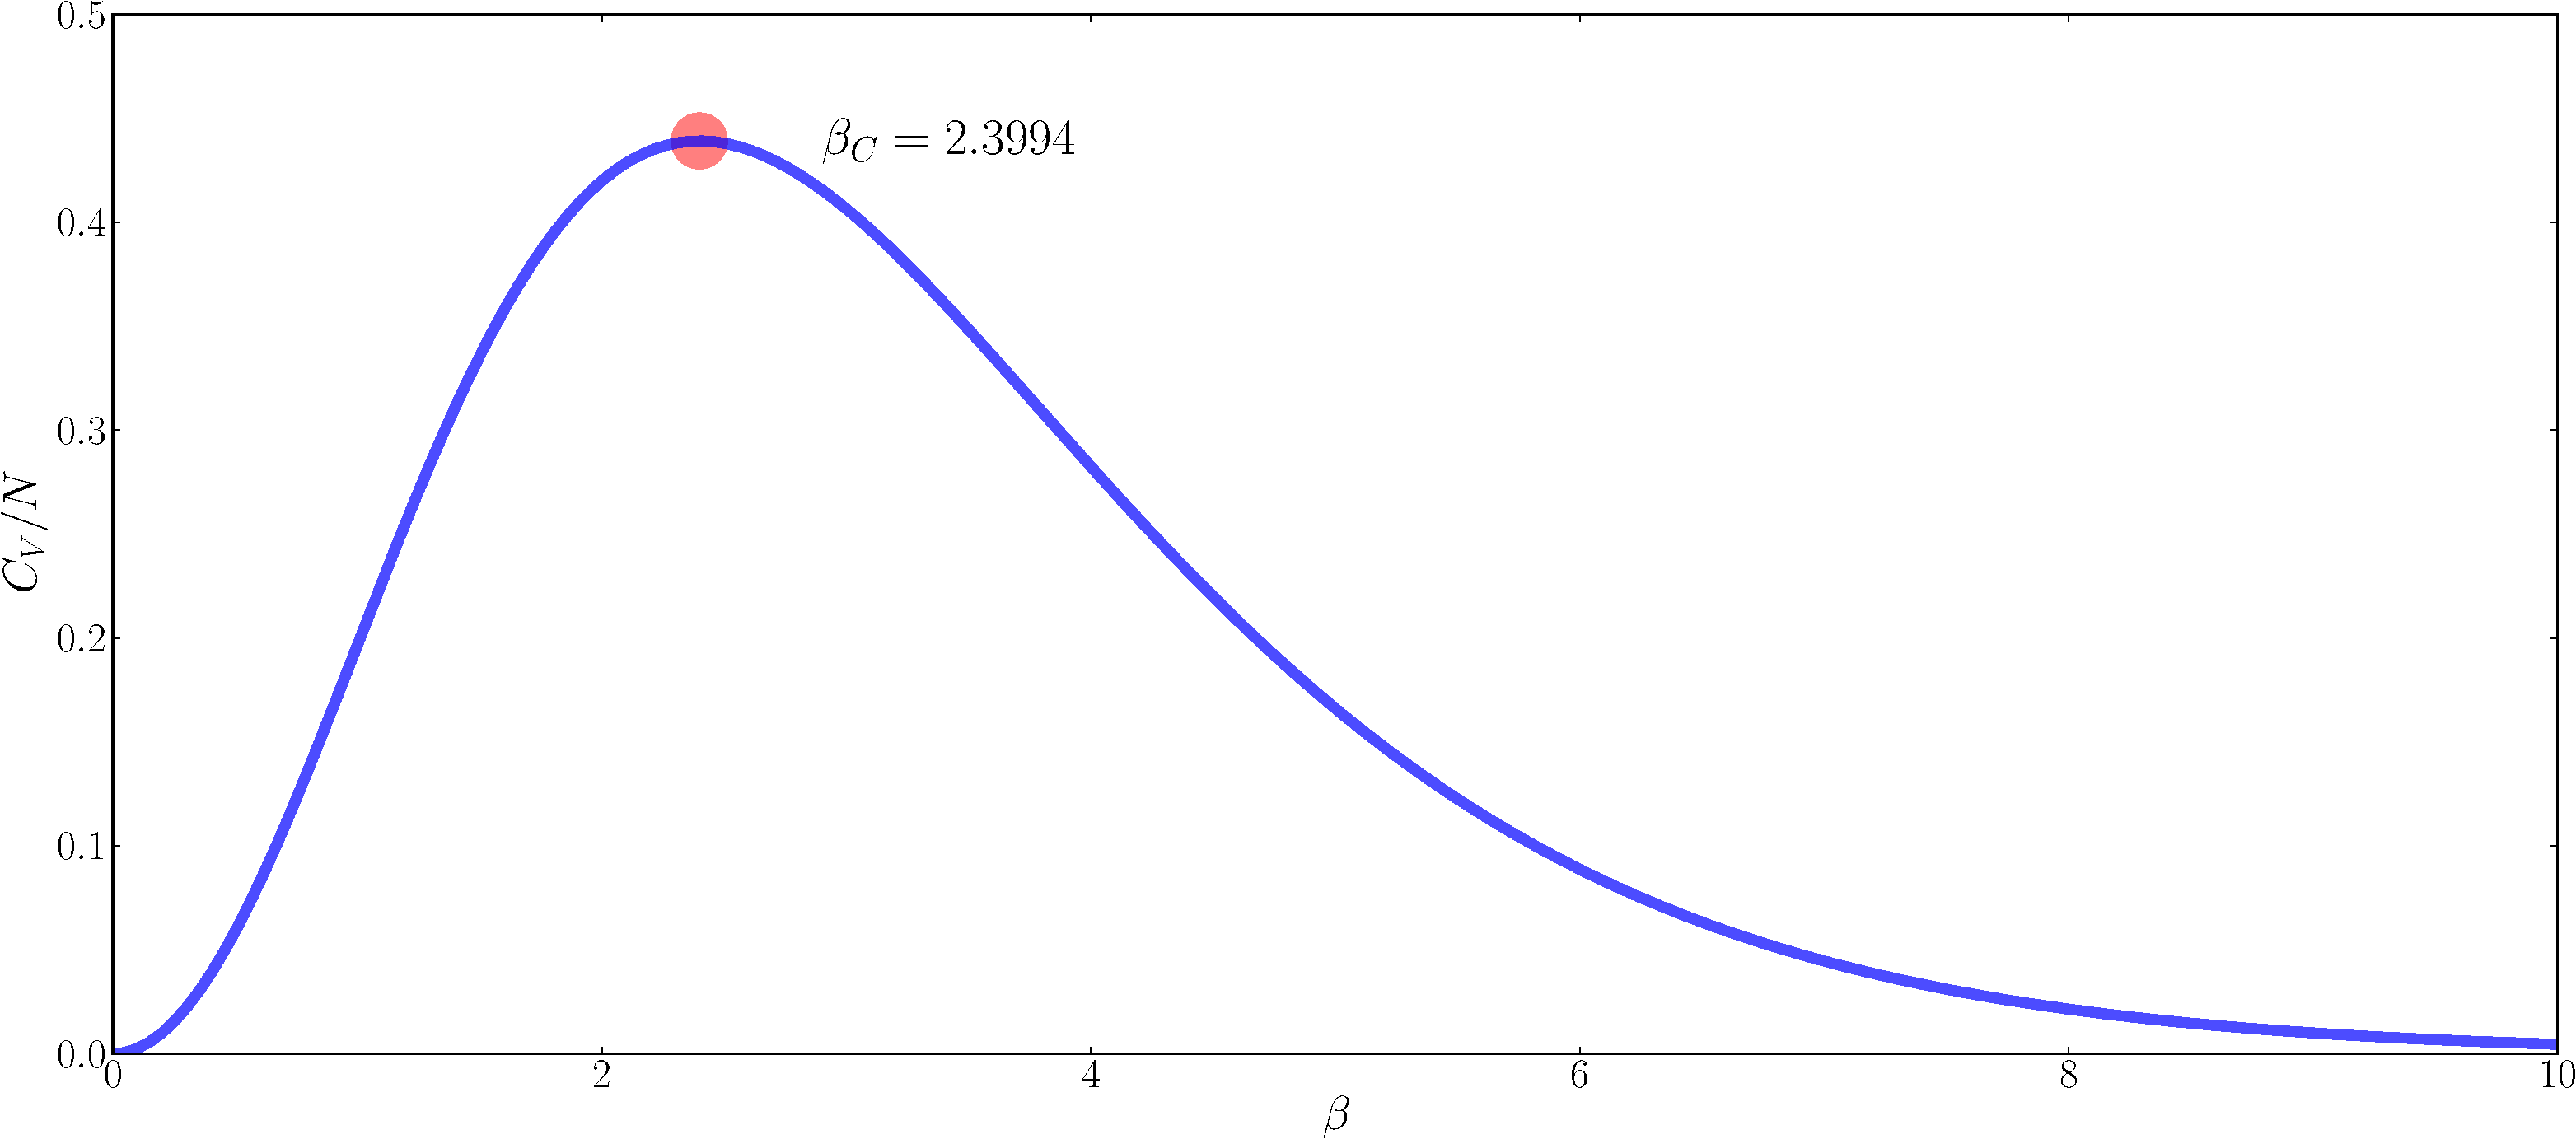
\includegraphics[width=.7 \textwidth]{pictures/1N_potts_ladder/pictures/CV_curve_potts_1N_ladder.pdf}
\caption{Specific heat per chain length for the one-dimensional Potts model with parameters $n=10^6$, $q=2$, and $J=-1$. The semi-critical $\beta$ was calculated from Equation \ref{eq:semi_critical_beta_potts_1N_ladder}. }
\label{fig:CV_curve_potts_1N_ladder}
\end{figure}
%

To visualize the behavior of the system on a larger scope, we can analytically continue the temperature onto the complex plane. In Figure \ref{fig:zeros_par_func_1n_ladder_no_field} we can visually inspect the behavior of the zeros on the complex plane. In the picture the semi-critical behavior (since we are plotting at finite $n$) is visible at $T=0$.

\begin{figure}[ht]
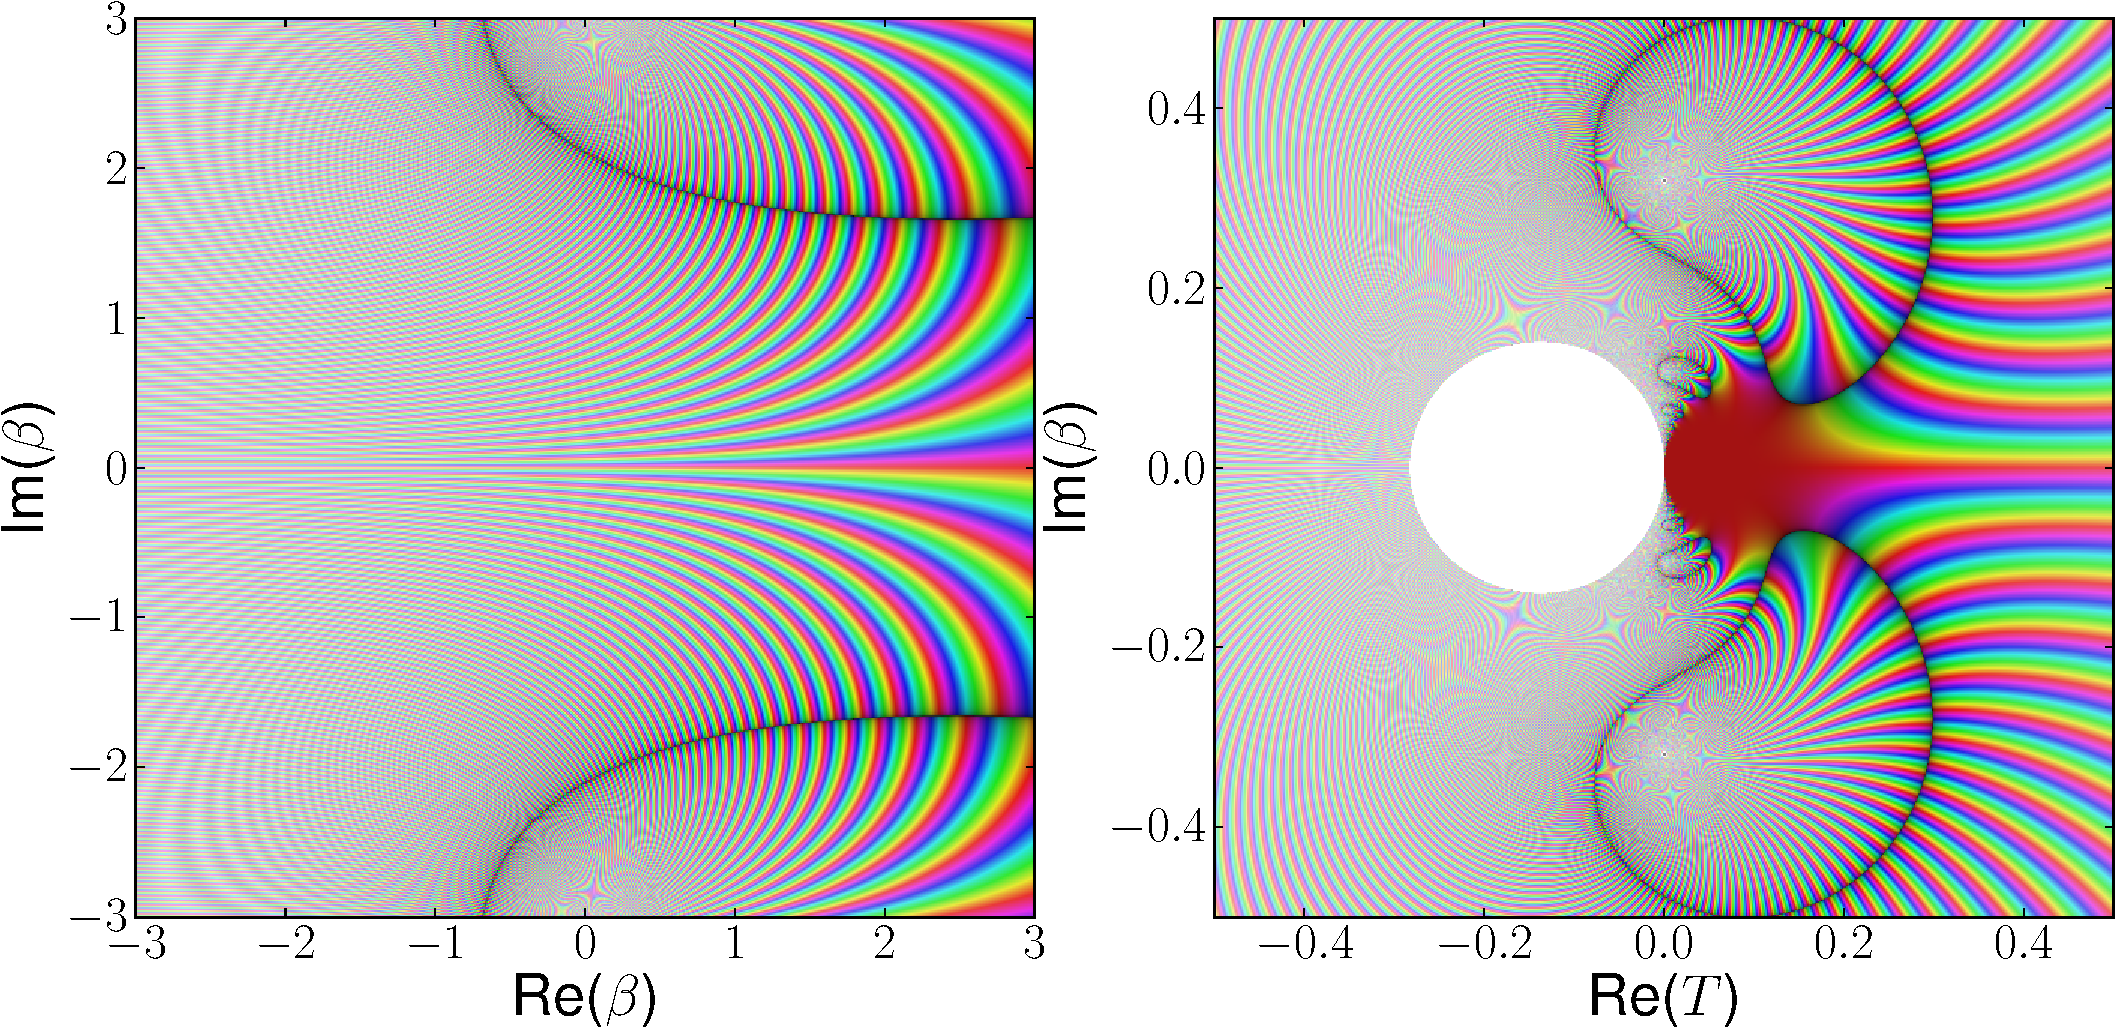
\includegraphics[width=\textwidth]{pictures/aggregation_model/pictures/zeros_parition_func_1N_ladder_2.pdf}
\caption{
Phase angle of the partition function for the $1N$ ladder with $J=-1$, $q=2$ where the temperature is continued onto the complex plane. The left plot has $\beta=1/kT$ to show the behavior of the high temperatures and the right plot shows the low temperature behavior. The points where the phase changes rapidly signify zeros of the partition function and hence first-order phase changes. The lighter areas on the low temperature plot are large values of the partition function (not zeros).
}
\label{fig:zeros_par_func_1n_ladder_no_field}
\end{figure}


\subsection{Special Case \texorpdfstring{$1N$}{1N} Ladder: Potts with Magnetic Field}

The standard Potts model with a field term only acting on the first state has the parameters of $w_j=w \delta(j,1)$ and $v_j=v$. This gives
\begin{align}
\CHI{a+1,}{a} 	&= w^{a+1}v^a + \sum_{j=2}^{q} v^a  
					 = w^{a+1}v^a + (q-1)v^a \\
X &= \sum_{n=0} y^n \CHI{n+1,}{n} 
   = {\frac{-w}{w v y-1}}-{\frac {q}{y v-1}}+ \frac{1}{y v-1}
\end{align}
Giving the generating function as
\begin{align}
Z(y) &=  {\frac { ( wvy-1 )  ( yv-1 ) }{{y}^{2}{v}^{2}w-y
v-w v y+1-w y+q w v{y}^{2}-y q+y}}
\end{align}
While resulting expression for $Z_n = \evalat{ \partial_y^n Z(y) } _ {y=0} $ is too complicated to evaluate explicitly, any particular term can be extracted with ease. 
\begin{comment}
To find semi-critical $\beta$ we look at the variance of the energy (where we substituted $v=e^{\beta J} -1$:
\begin{align}
\avg{ (\Delta E)^2 } &= 
\pfrac{^2 \ln(Z_n)}{\beta ^2} \\
&= {\frac { ( 1-q-n+nq ) {J}^{2}{{\rm e}^{\beta\,J}}}{ ({{\rm e}^{\beta\,J}}-1+q) ^{2}}}
\end{align}

Solving for the zeros of this function give:
\begin{equation}
\beta_c = \frac{\ln(q+1)}{J}
\end{equation}

Which when substituted into the specific heat $C_V = \beta^2 \avg{ (\Delta E)^2 }$, gives us the maximum value of the specific heat, a value independent of $J$ and $n$ for large values of $n$:
\begin{equation}
C_{V \text{max}} = \frac{\ln(q-1)^2 (n-1) }{4n} \approx \frac{\ln(q-1)^2 }{4}
\end{equation}

\end{comment}

\section{One-dimensional \texorpdfstring{$2N$}{2N}  Ladder }
\label{sec:two_d_ladder}

\begin{center}
\TIKZgraphtwoline
\end{center}

We give the general recurrence relation for the $2N$ ladder. The generating function solution remains an open problem. With a one dimensional strip two lattice units thick the operator is
\begin{equation}
\B{L} = 
\B{T}_{-2} \B{D}_2 \B{D}_1 
(\B{I} + \B{J}_{34}) 
(\B{I} + \B{J}_{13}) 
(\B{I} + \B{J}_{23}) 
\B{A}_{3} \B{A}_{4}
\end{equation}

There are now two general states which we have to consider. The first is when the vertices do not belong to the same partition $\ket{\pblock{1}{a_1}{b_1} \pblock{2}{a_2}{b_2} }$ and the second when they do belong to the same partition $\ket{\pblock{1 2}{a_3}{b_3}}$. We let $f_{a_1, b_1, a_2, b_2}$ and $g_{a_3, b_3}$ represent a shorthand for the two states respectively. The action of the operator is on $f$ is
\begin{align}
\B{L} f_{a_1, b_1, a_2, b_2} &= f_{a_1+1, b_1+1, a_2+1, b_2+1} 
											+ \CHI{a_1+1,}{b_1} f_{0,0, a_2+1, b_2+1} \\ \notag
                                	&+ \CHI{a_2+1,}{b_2} f_{a_1+1, b_1+1,0,0} 
                                	+ \CHI{a_1+1,}{b_1} g_{a_2+1,b_2+2} \\ \notag
                                	&+ \CHI{a_2+1,}{b_2} g_{a_1+1,b_1+2}
                                	+ g_{a_1+a_2+2,b_1+b_2+3} \\ \notag
                                	&+ \CHI{a_1+1,}{b_1} \CHI{a_2+1}{b_1} g_{0,1}
										  	+ \CHI{a_1+1,}{b_1} f_{0,0,0,0} 
\end{align}
And the action on $g$ is given by
\begin{align}
\B{L} g_{a_3, b_3}	&= f_{a_3+2, b_3+1, 0,0}
									+  f_{0,0,a_3+2, b_3+1} \\ \notag
									&+ 3g_{a_3+2,b_3+2}
									+  g_{a_3+2,b_3+3} \\ \notag
									&+ \CHI{a_3+2}{b_3} g_{0,1}
									+  \CHI{a_3+2,}{b_3} f_{0,0,0,0}
\end{align}
%
As before we let $\phi_n$ be the n\textsuperscript{th} application of $\B{L}$ against the initial state
\begin{equation}
\phi_n = \sum_{i,j \ge 0} c_{n, i, j} g_{i, j} + \sum_{i_1,i_2,j_1,j_2 \ge 0} d_{n, i_1,j_1,i_2,j_2} f_{i_1,j_1,i_2,j_2}
\end{equation}
with the initial state
\begin{equation}
\phi_0 = g_{0 1} + f_{0 0 0 0}
\end{equation}
We note that by symmetry we have
\begin{equation}
d_{n, i_1,j_1,i_2,j_2 } =  d_{n, i_2,j_2,i_1,j_1}
\end{equation}
%
Using that information we invert the equations
{
\allowdisplaybreaks
\begin{align}
c_{n01}&= \sum_{ij} \CHI{i+2,}{j} c_{n-1, i,j}   \\ \notag
		 &+ \sum_{i_1,i_2,j_1,j_2} \CHI{i_1+1,}{j_1} 
		 		\CHI{i_2+1,}{j_2} d_{n-1,i_1,i_2,j_1,j_2} \\ 
c_{nab} &= 3 c_{n-1, a-2,b-2} + c_{n-1, a-2,b-3} \\ \notag
		  &+ 2 \sum_{i,j} \CHI{i+1,}{j}  d_{n-1,i,j,a-2,b-2} \\ \notag
		  &+ 2 \sum_{i,j} d_{n-1,i,j,a-i-2,b-j-3} \\
d_{n a a00} &= c_{n-1, a-2,a-1} + S_1(a,a) + S_2(a) \\ \notag
d_{nab00} &= c_{n-1, a-2,b-1} + S_1(a,b) \\ \notag
d_{n,i_1,j_1,i_2,j_2} &= d_{n-1,i_1-1,j_1-1,i_2-1,j_2-1}
\end{align}
With
\begin{align}
S_1(a,b) &= \sum_{k=0}^{n-1} \CHI{k+1,}{k} d_{n-1-k,a-1-k,b-1-k,0,0} \\
S_2(a) &= \sum_{i=a}\sum_{j=a} \CHI{i+1,}{j} d_{n-a,i-a-1,j-a-1,0,0}
\end{align}
}

\section{Edge contraction methods}
\label{sec:edge_contraction_methods}

In the previous section we developed a method to determine the full partition function for an arbitrary graph with a field term using an operator expansion. While this is the most general method, it does limit the depth of the results one can obtain due to the complicated nature of the recursion relations. If we simplify the Hamiltonian by dropping the field term ($h=0$ in Eq. \ref{eq:potts_model_ham}), the solution to a wider class of graphs becomes tractable.

An equivalent evaluation to $\Z$ is the recursion relation mediated by graph reductions of edge contraction and removal (see Section \ref{sec:graph_introduction} for an explanation of these methods). There does not appear to be a general formula for the Potts model with an external field, but by relaxing this constraint there is the well-known relation\cite{godlin_graph_2008}
\begin{align}
\Z(G) &= w_{ij} \Z(G_{/ e_{ij}}) + \Z(G_{- e_{ij}}) \\
\Z(G_1 \sqcup G_2) &= \Z(G_1) \Z(G_2) \\
\Z(\emptyset) &= 1 \\
\Z(S) &= q
\end{align}
Here $/ e_{ij}$ is edge contraction, $-e_{ij}$ is edge removal, and $w_{ij}$ is the weight of the edge joined by vertices $i,j$. $G_1 \sqcup G_2$ represents two graphs that do not share any edges. $S$ is the singleton graph, with only one vertex and no edges and $\emptyset$ is the empty graph.

We can immediately derive the results for the $1N$ chain in the absence of an external field. As a pedagogical bonus, the resulting derivations can be done graphically. With a chain of length $n$, an edge weight of $v$ for each sequential vertex along the chain, the partition function for the n\textsuperscript{th} chain is
\begin{align}
Z(n) = \TIKZoneladderA
   & = v \paren{ \TIKZoneladderB }
+ \paren{ \TIKZoneladderC }
\\ \notag
& = v Z(n-1) + q Z(n - 1) 
\\ \notag
& = Z(n-1) (v + q)
\end{align}
%
Since the recursion relation is linear, it can be solved for in closed form giving exactly Equation \ref{eq:1N_ladder_potts_closed_form}.
\begin{align}
Z(n) &= q(v+q)^{n-1}
\end{align}

\subsubsection{$2N$ Ladder - Directional bonds}
We now attempt to solve the $2N$ chain with bond strengths that vary in along the short or long edge of the ladder. The strengths for the vertical and horizontal directions respectively are $J_1$ and $J_2$ (where $v_1=e^{J_1 \beta}-1$ and $v_2=e^{J_2 \beta}-1$)
{
\allowdisplaybreaks
\begin{align}
Z(n) &= \TIKZtwoladdera \\ \displaybreak[0]
     &= v_1 \TIKZtwoladderb + \TIKZtwoladderc \\ \displaybreak[0]
     &= v_1 v_2   \TIKZtwoladderd + Z(n-1) ( (v_2 + q)^2  + v_1(v_2 +q) ) \\ \displaybreak[0]
     &= v_1 v_2^2 \TIKZtwoladdere + Z(n-1) ( (v_2 + q)^2  + v_1(v_2 +q) + v_1 v_2 )  \\ 
     &= v_1 v_2^2  \TIKZtwoladderf  (1+ v_1) 
     + Z(n-1) ( (v_2 + q)^2  + v_1(v_2 +q) + v_1 v_2 )  
\end{align}
}
We notice however that the final graph is one that has already been seen before in the expansion, just shifted by one term in the recurrence
\begin{align}
Z(n-1)          &= v_1 \TIKZtwoladderf + Z(n-2) (v_2 + q)^2 \\
\TIKZtwoladderf &= \frac{1}{v_1} ( Z(n-1) - Z(n-2) (v_2 + q)^2) 
\end{align}
This gives the recursion relation of
\begin{equation}
Z(n) = Z(n-1)((q+v_2)^2+v_1(q+2v_2)) +  (Z(n-1)-Z(n-2)v_2^2 (q+v_2)^2(1+v_1)
\end{equation}
The initial conditions are
%
\begin{align}
Z(1) &= q(v_1 + q) \\
Z(2) &= ((v_1+q)(v_2+q))^2 - (v_1 v_2)^2 (q-1)
\end{align}
This again is a linear recurrence relation, albeit with two terms, that can be solved for rather easily. The closed form solution however is rather verbose and not particularly illuminating we provide the (slightly) more compact generating function
\epigraph{\begin{align}
Z(y) &= \frac{a}{b} 
\\ \notag a=& 
-y q(-y v_1v_2^2-y v_1v_2q-y v_1^2v_2-y q v_1^2-v_1-y q^2v_1-q+v_1^2v_2^2y+2y v_1v_2^2q
\\ \notag & \hspace{1em}
+ y v_1^2v_2q+y v_1v_2q^2+v_1^3v_2^2y+v_1^2v_2^2y q)
\\ \notag b=& 
v_1v_2^4y^2+v_1^2v_2^4y^2-2y v_2q-y v_1v_2-2y v_1v_2^2+1+2v_1v_2^3y^2q+2v_1^2v_2^3y^2q+
\\ \notag & \hspace{1em}
y^2v_1v_2^2q^2+v_1^2v_2^2y^2q^2-y v_1v_2q-y v_2^2-y q^2-v_1^2v_2^2y
\end{align}}{GF for 2N Ladder with no field term}

\begin{comment}
Using the closed form solution we can look for the discontinuities attempting to find phase transitions. The solutions for $v_1$ where $Z(n)=0$ are
\begin{align}
\text{critical}(v_{1c}) &=   
\{ -1, \rootof ((2v_2^2q+4v_2q+q^2+4v_2^2+v_2^4+4v_2^3)v_{1c}^2 + 
\\ \notag &
(-4v_2^3q+8v_2q^2-2q^2v_2^2+2q^3+12v_2^2q+8v_2^3)v_{1c}+4v_2q^3+4q^2v_2^2+q^4) \}
\end{align}
\end{comment}


Using the closed form solution we can look for the discontinuities attempting to find phase transitions. The solutions for $\beta$ where $Z(n)=0$ only have negative values for those on the real axis. It seems that the other roots also do not have real, positive solutions for $q \geq 2$, implying that the system has no mathematical phase transitions in the physical parameter space. This is best visualized in Figure \ref{fig:zeros_par_func_2nladder}.
%
\begin{figure}[hb]
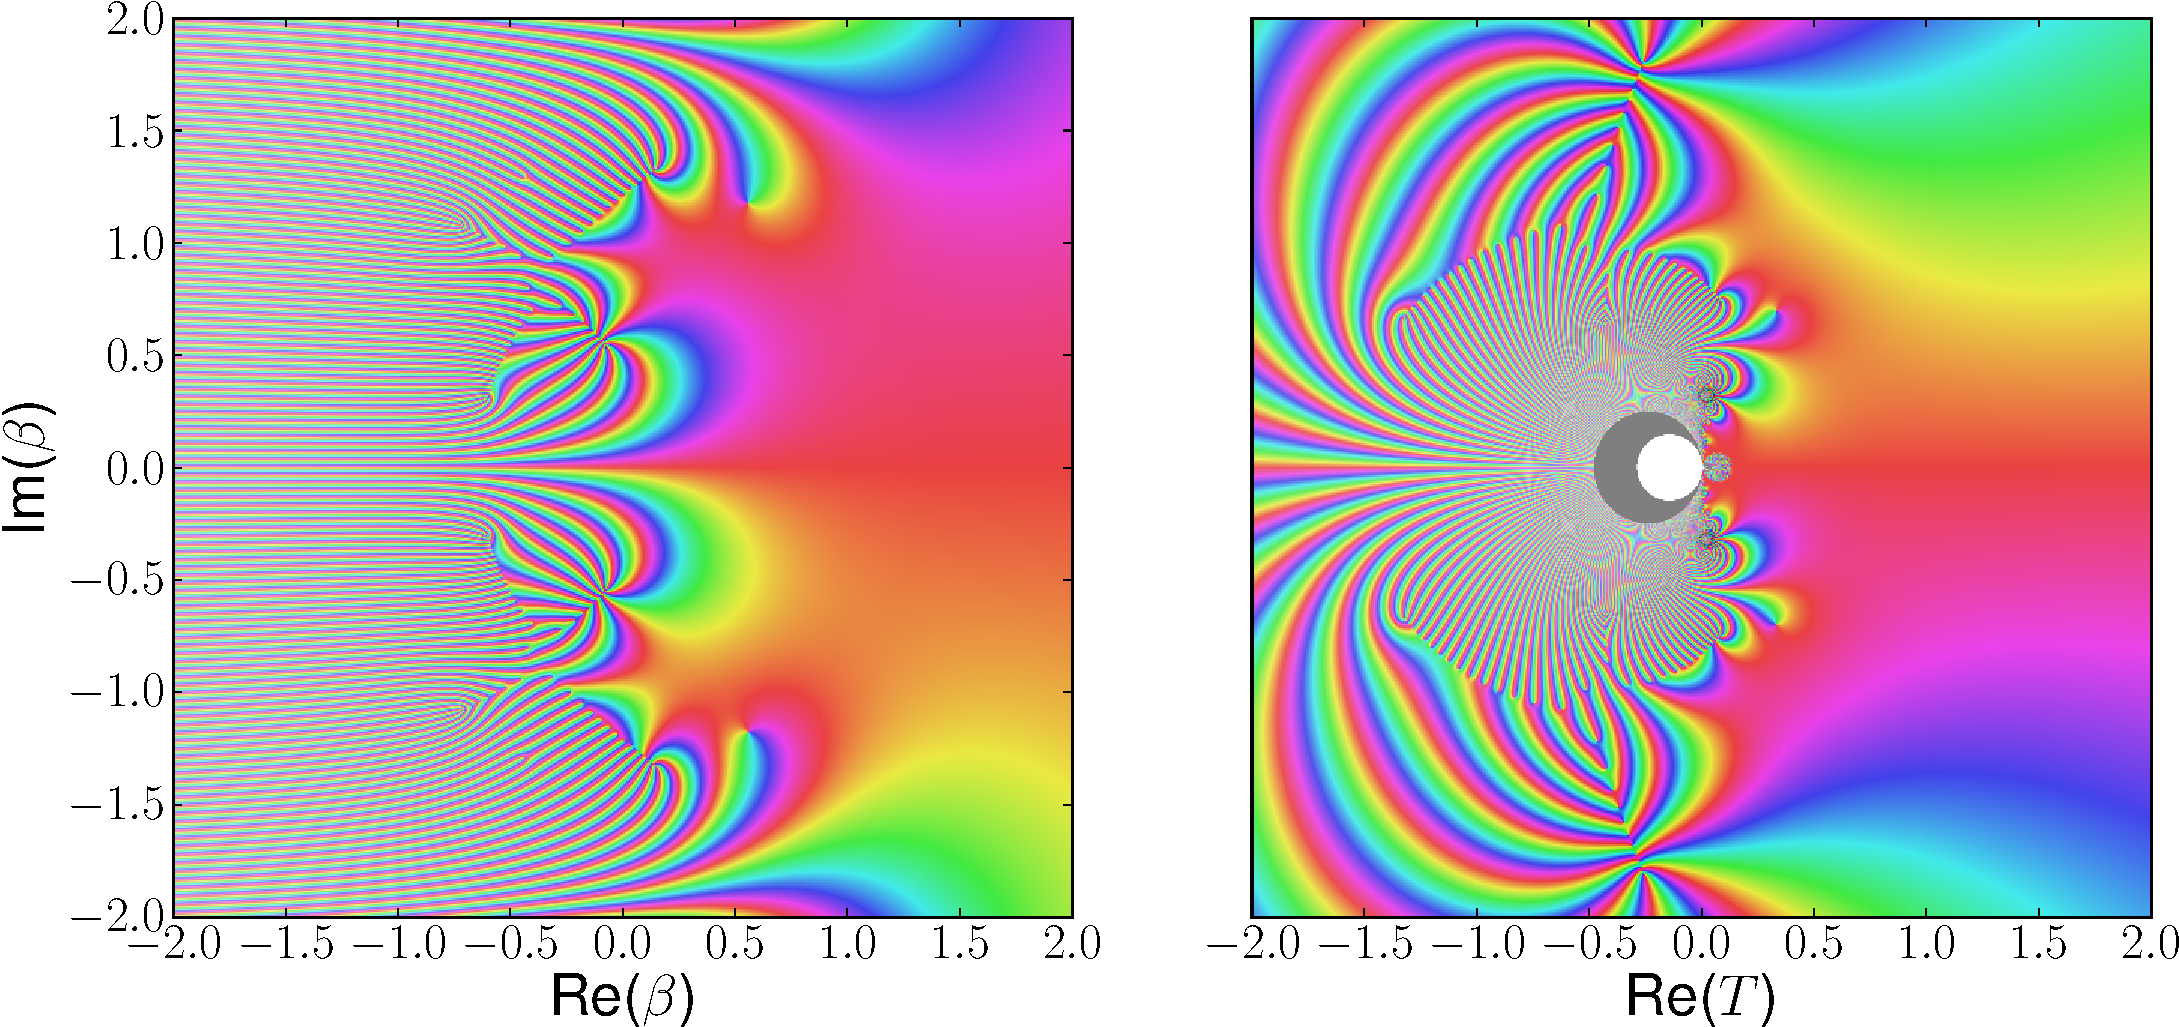
\includegraphics[width=\textwidth]{pictures/aggregation_model/pictures/zeros_parition_func_2N_ladder_2.pdf}
\caption{Phase angle of the partition function for the $2N$ ladder with $J_1=-2, J_2=-1$ where the temperature is continued onto the complex plane. The left plot has $\beta=1/kT$ to show the behavior of the high temperatures and the right plot shows the low temperature behavior. The points where the phase changes rapidly signify zeros of the partition function and hence phase changes. The gray areas and on the low temperature plot are large values of the partition function (not zeros) where the evaluation failed due to an overflow error. The lighter areas are large values of the partition function (not zeros).
}
\label{fig:zeros_par_func_2nladder}
\end{figure}

\begin{comment}
We can look at asymptotic large $n$ solutions by studying the poles of the generating function. The poles of the generating function $Z(y,n)$ are
\begin{align}
\{
\rootof (& 1+(v_2^4+v_2^4v_1+2v_2^3q+2v_2^3q v_1+q^2v_2^2+v_2^2q^2v_1)y_p^2
\\ \notag &
+(-2v_2^2-2v_2q-q^2-q v_1-2v_1v_2-v_2^2v_1)y_p)
\}
\end{align}
\end{comment}

\subsubsection{$3N$ Ladder - Directional bonds}
We give the general recurrence relations for a $3N$ ladder with bonds strengths that vary in direction. The strength for the vertical and horizontal directions respectively are again $J_1$ and $J_2$ where $v_1=e^{J_1 \beta}-1$ and $v_2=e^{J_2 \beta}-1$. It is to cumbersome to write the terms graphically in each equation, so we assign a symbol for each graph in the expansion indexed by the length of the ladder. 
{ \allowdisplaybreaks
\begin{tabular}{ c c c}
$Z(n)$            & $B(n)$               & $C(n)$ \\
\TIKZthreeladderA & \TIKZthreeladderB & \TIKZthreeladderC \\ 
$D(n)$               & $E(n)$               & $F(n)$ \\
\TIKZthreeladderD & \TIKZthreeladderE & \TIKZthreeladderF \\ 
$H(n)$               & $I(n)$               & $J(n)$ \\
\TIKZthreeladderH & \TIKZthreeladderI & \TIKZthreeladderJ \\ 
\end{tabular}
}
%
This gives a set of coupled recurrence relations
{ \allowdisplaybreaks
\begin{align}
Z(n) &= v_1 B(n) + (q+v_2) C(n) \\
C(n) &= v_1 D(n) + (q+v_2)^2 Z(n-1) \\
D(n) &= v_1 E(n) + (q+v_2) Z(n-1) \\
E(n) &= v_2(1+v_1) F(n) + Z(n-1) \\
B(n) &= v_1 G(n) + (q+v_2) D(n) \\
G(n) &= v_2 E(n) + (q+v_2)Z(n-1) + v_2 H(n) \\
H(n) &= v_2 I(n) + E(n) \\
I(n) &= v_2 (1+v_1)^2 G(n-1) + J(n) \\
J(n) &= v_1 (1+v_1) G(n-1)  + v_1 G(n-1) \\ \notag
     &\hspace{2em} + (v_2 + q)( Z(n-2)(1+ (v_2+q)) J(n-1) ) \\
F(n) &= B(n-1)
\end{align}
}
These equations could, in theory, be solved to get a recurrence relation on in terms of $\{ Z(n), Z(n-1), Z(n-2), \ldots \}$. We conjecture that the process could continue indefinitely for larger ladders, though we have not explored the $4N$ ladders or higher.

\section{Remarks}
%
In this chapter we developed new methods for solving the Ising/Potts model over arbitrary graphs and sought closed form solutions to ladder graphs. The ladder graphs have a natural connection to amyloid fiber aggregation with a preferred growth direction since one can take into account different bond strengths along each direction. These models permit only a few free parameters $J_1$, $J_2$, $q$ and for the graphs solved with external fields $h$. The results presented here open avenues of future work to connect the analytical models to concrete experimental data of real amyloid fiber growth by fitting these parameters.

